% a sample file for Journal of Quantum Information and Computation (QIC) in 
% LaTex2e by inputing macro file "qic.sty" with command \usepackage{qic}, 
% all the macros have been defined in the style file, so it is no need to 
% put many macros at the beginning of the text file  

\documentclass[twoside]{article}
\usepackage{qic,epsfig}
\usepackage{braket}
\usepackage{bm}
\usepackage{amssymb}
\usepackage{algorithm}
\usepackage{amsmath}
\usepackage{cancel}
\usepackage{qcircuit}
\usepackage{mathtools}
\usepackage{verbatim}
\usepackage{breqn}
\usepackage{algpseudocode} 
\usepackage{tikz}
\usepackage{url}
\usetikzlibrary{arrows.meta}

\textwidth=5.6truein
\textheight=8.0truein

\renewcommand{\thefootnote}{\fnsymbol{footnote}}  %use symbolic footnote

%%%%%%% starting the text file 

\begin{document}
\setlength{\textheight}{8.0truein}    %FOR 2ND PAGE ONWARDS

\runninghead{Mapping Fermions to Qubits  $\ldots$}
            {Oliver O'Brien $\ldots$}

\normalsize\textlineskip
\thispagestyle{empty}
\setcounter{page}{1}

%\copyrightheading{Vol.}{No.}{Year}{Page Nos.}

  

\alphfootnote

\fpage{1}

\centerline{\bf
%%%%%%%%%%%%%%%%%%%%%
%Put in titiles here
%%%%%%%%%%%%%%%%%%%%%
MAPPING FERMIONS TO QUBITS}
\vspace*{0.37truein}
\centerline{\footnotesize 
%%%%%%%%%%%%%%%%%%%%%%%%%%%%%%%%%%%%
%put authors' name and address here
%%%%%%%%%%%%%%%%%%%%%%%%%%%%%%%%%%%%
OLIVER O'BRIEN}
\vspace*{0.015truein}
\centerline{\footnotesize\it DAMTP, Centre for Mathematical Sciences, University of Cambridge, Cambridge CB30WA, UK}
\baselineskip=10pt
\centerline{\footnotesize\it Christ's College, Cambridge, UK}
\vspace*{0.225truein}
\publisher{(received date)}{(revised date)}

\vspace*{0.21truein} 

%% \abstracts{first paragraph}{second paragraph}{third paragraph}
%% If there is only one paragraph, just keep the second and third empty 
%% like the following one 
\abstracts{
%%%%%%%%%%%%%%%%%%%%
% put abstract here
%%%%%%%%%%%%%%%%%%%%
Your abstract goes here. 
}{}{}

\vspace*{10pt}

\keywords{The contents of the keywords}
\vspace*{3pt}
\communicate{to be filled by the Editorial}

\vspace*{1pt}\textlineskip    %) USE THIS MEASUREMENT WHEN THERE IS
   %) A SECTION HEADING
%\vspace*{-0.5pt}
%\noindent
%%%%%%%%%%%%%%%%%%%%%%%%%%%%%%%%
%put the text of the paper here
%%%%%%%%%%%%%%%%%%%%%%%%%%%%%%%%
\section{Introduction}
"Nature isn't classical, dammit, and if you want to make a simulation of nature, you'd better make it quantum mechanical, and by golly it's a wonderful problem, because it doesn't look so easy." - \textsl{Dr Richard Feynman} \cite{feynmann}  \\\\
Ever since Dr Richard Feynman spoke these famous words at the end of his keynote speech in 1982 one of the main tasks facing quantum computers has been simulating quantum systems. Intuitively a quantum computer should be able to handle this problem better than a classic computer as they operate within the same bizarre world of entanglement and superposition. However, there are many challenges to overcome before quantum advantage can be achieved in this field. We will consider one such challenge in this essay: the optimum mapping scheme from fermions to qubits.\\\\
One of the most common classes of quantum systems we wish to simulate are those composed of fermions. In order to simulate these particles we must find a representation for them a quantum computer can process; in terms of qubits and qubit operators. This poses a fundamental issue as fermions exhibit the non-local property of anti-commutation, whereas qubits are independent local systems. Therefore a non-trivial mapping scheme which introduces this non-local behaviour is necessary.\\\\
The first such mapping, the \textbf{Jordan-Wigner Transformation}, was invented nearly a century ago \cite{originalJordanWigner}, and we will introduce it in Section~\ref{jordan-wigner_section}. More recently, a number of new mappings have been developed including the \textbf{Bravyi-Kitaev map} and the \textbf{Derby-Klassen map}, which will be discussed in Section~\ref{bravyi-kitaev_section} and Section~\ref{derby-klassen_section} respectively. We will use three different formulations to explain the Bravyi-Kitaev mapping: partial ordering, transformation matrices and Fenwick Trees. Section~\ref{partialorderingsec} on partial ordering contains two original proofs of Bravyi-Kitaev's lemmas \cite{bravyikitaev}. Then, in Section~\ref{comparision_section} we compare the relative performance of these mappings in real-world applications (using simulated quantum computers).
\\\\
Recent research \cite{fermionicEncoding} has shown that the \textbf{fermionic enumeration} scheme used in the Jordan-Wigner mapping offers potential for increased locality with no additional resources. This is elaborated on in Section~\ref{fermionic-enumeration_section}.
\\\\
Finally, we have proposed a \textbf{new mapping} that combines aspects of the Jordan-Wigner and Bravyi-Kitaev mappings which we introduce in Section~\ref{novel}. This mapping is demonstrated to reduce gate count with less increased complexity than the Bravyi-Kitaev mapping.\\\\
It is important to consider how these mappings impact upon the fermionic simulation techniques used. Therefore, in Section~\ref{applications_section} (below) we will discuss how VQE and phase estimation can both be used to estimate the ground state energy of a system.
\section{Estimating ground state energies}\label{applications_section}
Computing the ground state energy of a Hamiltonian is generally the first step in computing the energetic properties of molecules and materials \cite{vqe}. Chemists have developed classical computational models for estimating the ground state, however, they all rely on approximations. Quantum computing opens up the potential for an exact (\textit{full configuration interaction}) approach, which is unfeasible on a classical computer where it scales exponentially in the number of fermionic modes. This section will consider two common approaches for estimating ground state energies on quantum computers (Variational Quantum Eigensolver and Quantum Phase Estimation) and how they are affected by the choice of fermion-to-qubit mapping.
\subsection{Variational Quantum Eigensolver (VQE)}\label{vqe_section}
A VQE provides an upper bound on the ground state energy of a Hamiltonian by utilising the variational principle:
\begin{equation}
        \frac{\bra{\psi} \hat H \ket{\psi}}{\braket{\psi | \psi}} \geq E_0 \>\>\>\> \forall \> \ket{\psi}\in \mathcal{H}
\end{equation}
The algorithm consists of two stages. First a variational ansatz $\ket{\psi}$ is initialised based on a set of parameters $\bm \theta$. Then, the Hamiltonian is measured a number of times, and the parameters of the ansatz are varied (using a classical optimiser) until a minimum is found. This is an example of a variational quantum algorithm, which performs a classical optimisation over a quantum oracle. By exporting lots of the work to a classical computer, VQEs are one of the quantum algorithms that are feasible in the NISQ (Noisy Intermediate-scale Quantum) era.\\\\ 
The preparation of ansatz can be done without any regard for fermions or specific mappings. Generally a given circuit structure is picked with some of the gates depending upon the parameters (i.e. an $R_z(\theta)$ gate). However, there are some ansatz which utilise a fermion-to-qubit mapping in the preparation of the state. One example of this is very commonly used Unitary Coupled Cluster (UCC) ansatz which is created by acting on a reference state with the exponential of a parametrised set of fermionic creation and annihilation operators (defined later in Section~\ref{secondquantization}). Therefore, this ansatz relies upon using a mapping (such as in Section~\ref{mapping}) to represent these operators as Pauli-strings (strings of Pauli operators). Exponentiating these, potentially non-commuting, Pauli-strings is non-trivial and requires the Trotter-Suzuki approximation (explored in more detail later in Section~\ref{trotter}). In summary, we only need to consider the impact of the mapping upon the preparation of the ansatz if the mapping is explicitly invoked by the particular preparation used. This essay will not consider such preparations.\\\\
It is in the measurement of the Hamiltonian that the mapping is always important. Using the second quantization (discussed in Section~\ref{secondquantization}), the Hamiltonian will be a combination of fermionic raising and lowering operators, so needs to be mapped to a combination of Pauli operators that can be measured on a quantum computer. After this mapping has been performed we are left with a qubit Hamiltonian that is a sum of Pauli strings. Therefore, we can measure the effectiveness of different mappings by the resource costs of implementing this qubit Hamiltonian. We will focus on three metrics:
\begin{romanlist}
\item \textbf{Number of qubits:} The less qubits required by the mapping the smaller the quantum computer required to run the simulation.
\item \textbf{Average Pauli weight:} The average number of Pauli operators in each Pauli string in the Hamiltonian. The smaller the Pauli weight the less gates needed to measure the Hamiltonian, which reduces both the resource cost and the error due to gate infidelity. Reduced Pauli weights means a more local mapping with less qubits involved in each operation. Therefore, it allows for a greater level of parallelisation of operations which in turn reduces circuit (and ansatz) depth. Reduced circuit depth reduces the error due to decoherence. It has also been shown \cite{barrenplat} that lower Pauli weights provide some protection against barren plateaus (when the cost function has vanishing gradients), and so give more trainable cost functions. 
\item \textbf{Number of Pauli-strings:} Each Pauli-string is measured separately, so the fewer Pauli-strings to measure, the fewer times the ansatz needs to be initialized and measured.
\end{romanlist}
\subsection{Quantum Phase estimation (QPE)} \label{qpe_section}
QPE can be used to estimate the energy levels of a Hamiltonian to $n$ bits. This is achieved by applying successive steps of time evolution as a controlled gate with the target being the input state and the control being successive Hadamard ancilla qubits (illustrated in Fig.~\ref{QPECircuit}). Then by performing an inverse Quantum Fourier Transform on these ancilla qubits we get a superposition of binary expressions for the energy levels.\\
\begin{figure}[htbp]
               \centerline{ \Qcircuit @C=1em @R=.7em {
                               \lstick{\ket{0}} & \gate{H} & \qw            & \qw              & \qw              & \qw              & \qw &  \cdots &                & \ctrl{8}           & \qw & \multigate{7}{QFT^{-1}} & \qw \\ \\ \lstick{\cdots} & \cdots  & \cdots & \cdots & \cdots &\cdots &  & \cdots & &  & \cdots& & \cdots  \\   \\
                               \lstick{\ket{0}} & \gate{H} & \qw            & \qw              & \qw              & \ctrl{4}         & \qw &  \cdots &                & \qw                & \qw & \ghost{QFT^{-1}}& \qw  \\
                               \lstick{\ket{0}} & \gate{H} & \qw            & \qw              & \ctrl{3}         & \qw              & \qw &  \cdots &                & \qw                & \qw & \ghost{QFT^{-1}}& \qw   \\
                               \lstick{\ket{0}} & \gate{H} & \qw            & \ctrl{2}         & \qw              & \qw              & \qw &  \cdots &                & \qw                & \qw & \ghost{QFT^{-1}}& \qw   \\
                               \lstick{\ket{0}} & \gate{H} & \ctrl{1}       & \qw              & \qw              & \qw              & \qw &  \cdots &                & \qw                & \qw & \ghost{QFT^{-1}}& \qw   \\
                               \lstick{\ket{u}} & \qw      & \gate{U^{2^0}} & \gate{U^{2^{1}}} & \gate{U^{2^{2}}} & \gate{U^{2^{3}}} & \qw &  \cdots &                & \gate{U^{2^{n-1}}} & \qw & \qw & \qw
        }}
        \vspace*{13pt}
        \fcaption{\label{QPECircuit} Circuit diagram of QPE. In order to calcualte energy levels $U = e^{-2\pi i \hat H}$ is used.}
\end{figure} \\
The following explanation, adapted from \cite{chemistryReview}, illustrates in detail how these steps give the ground state energy:\\
\begin{itemlist}
\item We can express $\ket{u}$ in the basis of energy eigenstates: $\ket{u} = \sum_i c_i \ket{\phi_i}$ with $\hat H \ket{\phi_i} = E_i \ket{\phi_i}$. Therefore, the total state after the application of the Hadamard gates is: 
        \begin{equation}
                \frac{1}{\sqrt{2^n}} \sum_i \sum_x \ket{x} c_i \ket{\phi_i}
        \end{equation}
\item After the application of the controlled gates shown in Fig.~\ref{QPECircuit}, this transforms to:
        \begin{equation}
        \frac{1}{\sqrt{2^n}} \sum_i c_i (\ket{0} + e^{-2\pi i  E_i 2^0}\ket{1})(\ket{0} + e^{-2\pi i E_i 2^1} \ket{1}) \cdots (\ket{0} + e^{-2\pi i  E_i 2^{n-1}}\ket{1}) \ket{\phi_i} \end{equation}
        as $x = x_0 2^0 + x_1 2^1 + \cdots + x_{n-1} 2^{n-1}$ for $x_i \in \{0,1\}$, this reduces to:
        \begin{equation}
                \frac{1}{\sqrt{2^n}} \sum_i \sum_x e^{-2\pi i E_i x}c_i \ket{x}  \ket{\phi_i}
        \end{equation}
\item By applying an inverse Fourier transform the phase can be extracted:
        \begin{equation}
\frac{1}{\sqrt{2^n}} \sum_i \sum_x e^{-2\pi i E_i x}c_i \ket{x}  \ket{\phi_i} \xrightarrow{QFT^{-1}} \sum_i c_i \ket{E_i} \ket{\phi_i}
        \end{equation}
\item As $E_i$ is likely not exact to $n$ bits there will be a potential error introduced by the Quantum Fourier Transform, so to be accurate to $n$ bits a few more ancilla qubits will be needed \cite{nielsenChuang}.
\item By measuring the ancilla bits in the Z basis we will observe $E_i$ to $n$ bits with probability $|c_i|^2$.  So to find the ground state energy level, the ground state eigenstate needs to be in the original expansion of the guiding state $\ket{u}$. The larger the amplitude of the ground state eigenstate ($c_0$) the fewer repetitions of QPE are required before $E_0$ is measured. Therefore, QPE works better if a guiding state close to the exact ground state is used. To this end similar ansatz to those described in the previous section are used as guiding states. Therefore, it is only necessary to consider the impact of mapping upon preparation of guiding states if the mapping is involved in the preparation. This essay will not consider such preparations.\end{itemlist}
The portion of this algorithm for which fermionic mapping is always relevant is the construction of the controlled gates $U^{2^k} = e^{-2 \pi i \hat H 2^k}$. Not only do the same metrics for the efficiency of the corresponding qubit Hamiltonian listed in Section~\ref{vqe_section} apply, now we need to consider the impact of exponentiation. As the Hamiltonian is the sum of non-commuting Pauli-strings taking the exponential is non-trivial and requires the Trotter-Suzuki approximation \cite{suzuki}:
\subsection{Trotter-Suzuki approximation}\label{trotter}
To first order the Trotter-Suzuki approximation gives:
\begin{equation}
        e^{\frac{-it}{\hbar} \sum^m_k \hat H_k} = \left( \prod^m_k e^{\frac{-i t \hat H_k}{\hbar S}}\right)^S + O(m^3 t^2/S)
\end{equation}
In order to achieve a desired accuracy of $\epsilon$ a sufficient number of Trotter steps $S= O(t^2/ \epsilon)$ need to be used \cite{chemistryReview}. The ordering of the terms in this Trotter-Suzuki expansion influences the error and therefore how many Trotter steps are required. This is important to consider as the impact the ordering has varies depending on the mapping chosen as we will discuss in Section~\ref{comparision_section}.\\\\
Finally, it is useful to consider how each Trotter step is represented as a circuit. First, we consider that $e^{i(Z_1 \otimes Z_2 \otimes ... \otimes Z_n)\theta}$ applies a phase shift of $e^{i\theta}$ if the parity of the $n$ qubits is even and $e^{-i\theta}$ if the parity is odd. Therefore, in order to apply this operation we first compute the parity using a chain of CNOT gates, then apply $R_z(2 \theta)$, and the uncompute the parity with another chain of CNOT gates. There is now a phase difference of $2 \theta$ between odd and even parity, so this is equivalent (up to a global phase) to applying $e^{i ( Z_1 \otimes \ldots Z_n) \theta}$. Secondly, it is possible to transform $e^{i(Z_1 \otimes Z_2 \otimes ... \otimes Z_n)\theta}$ into the exponentiation of any Pauli-string by applying $R_X$ or Hadamard gates to change the basis to the X or Y basis, respectively. Therefore, in general the exponential of a $n$-fold tensor product of Pauli matrices will require $2(n-1)$ CNOT gates centred around one phase-shift gate and enough $R_X$ and Hadamard gates to transform into and out of the necessary basis before and after \cite{seeley}. As an example the circuit required for computing the term $e^{i(YXZY)\theta}$ is shown in Fig.~\ref{trotterStepCircuit}. As such it is clear that each Trotter step requires $O(mn)$ gates were $m$ is the number of Pauli strings and $n$ is the average Pauli weight of these strings.
\begin{figure}[htbp]
\centerline{ \Qcircuit @C=1em @R=.7em {
        &\gate{R_X} & \ctrl{1} & \qw & \qw & \qw & \qw & \qw & \ctrl{1} & \gate{R_X^{\dagger}}&\qw \\
        &\gate{H} & \targ & \ctrl{1} & \qw & \qw & \qw & \ctrl{1} & \targ & \gate{H}& \qw\\
        & \qw & \qw & \targ & \ctrl{1} & \qw & \ctrl{1} & \targ & \qw & \qw &  \qw\\
        &\gate{R_X} & \qw & \qw & \targ & \gate{R_Z(2 \theta)} & \targ & \qw & \qw & \gate{R_X^{\dagger}} &\qw \\
}}
        \vspace*{13pt}
        \fcaption{\label{trotterStepCircuit} The circuit required to exponentiate the Pauli-string $YXZY$ by first converting the qubits into the correct basis using $R_X$ and $H$ gates, then computing the parity of the four qubits before applying a single-qubit phase rotation. After this we uncompute the parity and revert to the computational (Z) basis. This is adapted from \cite{seeley}.}
\end{figure}
\section{First and second quantization}
This section builds up an explanation of second quantization which is the foundation of all the mappings explained later in the essay. A brief description of first quantization is given to illustrate another way of quantising qubits, and to highlight that fermionic creation and annihilation operators are simply a mathematical construction defined by their anti-commutation relations and/or their action on the Fock basis.
\subsection{First quantization}
From Quantum Field Theory (\textbf{citation needed}), it is known that fermions must be antisymmetric under exchange. This property is commonly represented by qubits in two ways known as the first and second quantization. The first quantization is when the antisymmetry is retained in the wavefunction such as with:
\begin{equation}\label{antisym}
        \ket{\Phi} = \frac{1}{\sqrt{2}}(\ket{\phi_1}_1 \ket{\phi_2}_2 - \ket{\phi_2}_1 \ket{\phi_1}_2)
\end{equation}
\begin{equation}\label{antisymwave}
        \Phi(\bm x_1, \bm x_2) = \frac{1}{\sqrt{2}}(\phi_1(\bm x_1) \phi_2(\bm x_2) - \phi_2(\bm x_1) \phi_1(\bm x_2))
\end{equation}
We can generalise Eq.~\ref{antisymwave} to larger numbers of fermions through a Slater determinant (Eq.~\ref{slater}) \cite{chemistryReview}. This satisfies the antisymmetry condition as swapping any two rows of a determinant produces a sign change:
\begin{equation}\label{slater}
        \phi(\bm x_0, ..., \bm x_{N-1}) = \frac{1}{\sqrt{N!}} 
        \begin{vmatrix} 
                \phi_0(\bm x_0) & \cdots & \phi_{M-1}(\bm x_0)\\
                \vdots & \ddots & \vdots \\
                \phi_0(\bm x_{N-1}) & \cdots & \phi_{M-1}(\bm x_{N-1})
        \end{vmatrix}
\end{equation}
where $M$ is the number of fermionic modes (e.g. spin orbitals) possible and $N$ is the number of particles (e.g. electrons). Typically we have more modes than particles, so the Slater determinant will only contain the $N$ occupied modes.\\\\ 
 In the first quantization the Hamiltonian is defined in terms of $\ket{\phi_p}\bra{\phi_q}$ \cite{tilly}, as in the example given by Eq~\ref{firstham}:
\begin{equation}
        \label{firstham}
        H = \sum_{p, q} \sum_i h_{pq}  \ket{\phi_p}_i \bra{\phi_q}_i + \frac{1}{2} \sum_{p,q,r,s}\sum_{i,j} h_{pqrs} \ket{\phi_p}_i \ket{\phi_q}_j \bra{\phi_r}_i \bra{\phi_s}_j
\end{equation}
As $\ket{\phi_p}\bra{\phi_q}$ commute, the operators can be considered to be symmetric. Therefore, the fermionic property of antisymmetry under exchange must be enforced by the wavefunctions they act upon and so must be directly included in the qubit representation of the wavefunction. Hence, the initial state will typically include $N$ registers (one per particle) of size $\log M$ (to encode the indices of occupied modes) in such a manner that the state is antisymmetric under exchange of any two of the $N$ registers. Some methods for creating such states are described in \cite{firstech1} and \cite{firstech2}, and involve using at least $O(N \log N)$ ancilla qubits \cite{firstech2} to count the number of exchanges required to sort a given set of $N$ registers. As such, first quantization generally requires $O(N \log M)$ qubits \cite{tilly} to encode the wave function.
\subsection{Second quantization} \label{secondquantization}
The second quantization compresses the information of the Slater determinant by only tracking whether each orbital or fermionic mode is occupied. Therefore Eq.~\ref{slater} is written as:
\begin{equation}
        \phi(\bm x_0, ..., \bm x_{N-1}) = \ket{f_0,\cdots, f_i, \cdots, f_{M-1}}
\end{equation}
where $f_i$ (the occupation number) $ =1$ when $\phi_p$ is occupied, and 0 otherwise. This is termed the Fock basis. In the second quantization the Hamiltonian is redefined in terms of fermionic creation ($a^{\dagger}_p$) and annihilation ($a_p$) operators, as shown in the example given by Eq.~\ref{secham}. These operators reintroduce the antisymmetry lost when compacting the Slater determinant by describing how to move between different occupation numbers \cite{chemistryReview} (illustrated by Eq.~\ref{secondQuant}):
\begin{equation}
        \label{secham}
        H = \sum_{p,q} h_{pq}a_p^{\dagger} a_q + \frac{1}{2}\sum_{p,q,r,s} h_{pqrs} a_p^{\dagger} a^{\dagger}_q a_r a_s
\end{equation}
\begin{equation}
        \label{secondQuant}
        \begin{align}
        a_p \ket{f_0,\cdots, f_i, \cdots, f_{M-1}} = \delta_{f_p, 1} (-1)^{\sum_{i=0}^{p-1} f_i} \ket{f_0,\cdots, f_p \oplus 1, \cdots, f_{M-1}}\\
        a_p^{\dagger} \ket{f_0,\cdots, f_i, \cdots, f_{M-1}} = \delta_{f_p, 0} (-1)^{\sum_{i=0}^{p-1} f_i} \ket{f_0,\cdots, f_p \oplus 1, \cdots, f_{M-1}}
\end{align}
\end{equation}
It is clear that Eq.~\ref{secondQuant} is equivalent to defining the fermionic creation and annihilation operators in terms the following commutation relations:
\begin{equation}
        \{ a_p, a_q^{\dagger}\} = \delta_{pq}, \{ a_p, a_q \} =  \{a^{\dagger}_p, a^{\dagger}_q\} = 0
\end{equation}
where $\ket{0,\ldots,0}$ is defined as the state such that $a_p \ket{0,\ldots,0} = 0$ for all $p$.\\\\
Therefore, using second quantization techniques the antisymmetry is enforced entirely by the operators rather than the state representation. This means far fewer qubits are needed compared to first quantization, especially as first quantization requires ancilla qubits of a similar order to the working set representing a significant overhead in the NISQ era. Therefore, the focus of research and the most common choice of quantization has been the second. However, it should be noted that the first quantization could be useful in systems with much fewer particles than possible modes ($N<<M$) \cite{tilly}, as then it would only require $O(\log M)$ qubits. 
\section{Mappings} \label{mapping}
When working with second quantization there is a lot of choice about how to optimally map the Fock basis and fermionic operators to qubits and Pauli operators. This section will explore three of these mappings: the Jordan-Wigner transformation, the Bravyi-Kiteav mapping and the Derby-Klassen mapping (as an example of a `local' mapping).\\\\
Each of these mappings has a different way of solving the problem of how to introduce the non-local property of antisymmetry, and they are each based upon the second quantization described in Section~\ref{secondquantization}. This section is primarily focused on presenting the mechanisms for the mappings; a detailed analysis of their relative performance is given in Section~\ref{comparision_section}.
\subsection{Jordan-Wigner Transformation}\label{jordan-wigner_section}
The first fermion to qubit mapping developed was the Jordan-Wigner transformation which straightforwardly stores the occupation number of the $i$-th orbital in the $i$-th qubit. Therefore, all the non-local behaviour (the parity information) has to be encoded in the operators \cite{fermionicEncoding}:
\begin{equation}
        \begin{align}
        a_i \rightarrow \left( \bigotimes_{k=1}^{i-1} Z_k \right) \sigma_i^-\\
        a^{\dagger}_i \rightarrow \left( \bigotimes_{k=1}^{i-1} Z_k \right) \sigma_i^+
\end{align}
\end{equation}
where
\begin{equation}
        \begin{align}
                \sigma^-_i = \frac{1}{2} (X_i + i Y_i) = \ket{0}_i \bra{1}_i\\
                \sigma^+_i = \frac{1}{2} (X_i - i Y_i) = \ket{1}_i \bra{0}_i 
        \end{align}
\end{equation}
The $\bigotimes_{k=1}^{i-1} Z_k$ term is necessary to apply the parity phase shift $(-1)^{\sum_{k=0}^{i-1} f_k}$. Therefore, it is clear that these operators act in exactly the same way on a qubit spin basis that the fermionic creation and annihilation operators act upon the Fock basis (Eq.~\ref{secondQuant}).
\subsection{Bravyi-Kiteav Map}\label{bravyi-kitaev_section}
The Jordan-Wigner transformation uses O(1) qubits to represent each fermionic mode, however it requires O(N) gates to simulate one fermionic operation. This is because it stores the occupation number locally and the parity non-locally. An alternative scheme called the parity basis\fnm{a} stores the parity locally and the occupation number non-locally, however this still requires O(N) gates to simulate one fermionic operation \cite{seeley}. The Bravyi-Kiteav is a halfway house which partially stores both the occupation number and parity non-locally.
\fnt{a}{In the parity basis the $i$-th qubit stores the parity $\sum_{j=0}^{i}f_j$. Therefore, it is the mirror of the Jordan-Wigner transformation with operators:
$$        a_i \rightarrow \left( \bigotimes_{k=i}^{n} \sigma_k^- \right) Z_{i-1} \>\>\>\> a^{\dagger}_i \rightarrow \left( \bigotimes_{k=i}^{n} \sigma_k^+ \right) Z_{i-1} $$}
\\\\
Bravyi and Kitaev first proposed this mapping as a way of simulating qubits using local fermionic modes and vice versa. In their original formulation they used a partial ordering scheme based on the representation of the fermionic modes in binary. Later, a scheme using transformation matrices was introduced \cite{seeley}, and it was noted in \cite{operatorLocality} that the partial ordering scheme can be considered in terms of Fenwick trees. We will illustrate all three of these approaches to give the broadest understanding of this mapping. 
\subsubsection{Partial ordering formulation}\label{partialorderingsec}
The following explanation in terms of partial ordering is adapted from \cite{bravyikitaev}: \\\\First, we must define a partial order $\preceq$ over a set of binary strings. For $\alpha = \alpha_{l-1}\ldots \alpha_0$ and $\beta = \beta_{l-1}\ldots \beta_0$, if $\alpha_i = \beta_i$ for $i\geq i_0$ and $\beta_i = 1$ for $i < i_0$, then $\alpha \preceq \beta$. For example:
$$
\begin{rcases}
        \begin{aligned}
        \begin{rcases}
                \begin{aligned}
                        000 \prec \>&001 \\
                                  &010
               \end{aligned}
       \end{rcases} \prec \>&011 \\
        100 \prec \>&101\\
                  &110
        \end{aligned}
\end{rcases}
\prec 111
$$
For the $i$-th qubit we store the parity of all modes $f_k$ with $k \preceq i$:
\begin{equation}
        q_i = \sum_{k \preceq i} f_k \label{paritystore}
\end{equation}
Before continuing with this discussion and defining the Bravyi-Kitaev operators we first must state and prove two results from \cite{bravyikitaev}:\\\\
{\bf Lemma~1 \cite{bravyikitaev}:} Define the set $L(\alpha)$ such that $\beta \in L(\alpha)$ if and only if for some $i_0$: $\alpha_{i_0} = 1$, $\beta_{i_0} = 0$, $\beta_i = \alpha_i$ for $i> i_0$ and $\beta_i = 1$ for $i< i_0$, then:
\begin{equation}
        \sum_{j \in L(i)} q_j = \sum_{j < i} f_j
\end{equation}
\vspace*{12pt}

\noindent
The following proof is of my own invention:
\begin{equation}
L(\alpha) = \{ \alpha_{n-1} \ldots \alpha_{i_0 +1} 0 11 \ldots 1: \forall \>i_0\text{ s.t. } \alpha_{i_0} = 1\}
\end{equation}
Define $A(\beta)$ as the set of $j$ such that $j \preceq \beta$:
\begin{equation}
        A(\beta) = \{j: j \preceq \beta\} 
\end{equation}
\begin{equation}
        \label{AL}
A(L(\alpha)) =  \{\{  j: j \preceq \alpha_{n-1} \ldots \alpha_{i_0+1}0 1 \ldots 1 \} \forall i_0 \text{ s.t. } \alpha_{i_0} = 1 \}
\end{equation}
As $A(\alpha_{n-1}\ldots\alpha_{i_0+1}01\ldots11) =  \{j:\alpha_{n-1}\ldots \alpha_{i_0+1} 0\ldots 00\ \leq j \leq \alpha_{n-1}\ldots \alpha_{i_0+1} 01\ldots 11\}$, Eq.~\ref{AL} is an algorithm for generating the set of all the integers less than $\alpha$. Moving from left to right at every $\alpha_{i_0}= 1$ we generate the set of integers $[\alpha_{n-1}\ldots\alpha_{i_0+1} 0\ldots0, \alpha_{n-1} \ldots \alpha_{i_0+1}10 \ldots 0)$. 
$$\bigcup_{S\in A(L(\alpha))}S = \bigcup_{\alpha_{i_0} = 1} \{j:\alpha_{n-1}\ldots \alpha_{i_0+1} 0\ldots 00\ \leq j < \alpha_{n-1}\ldots \alpha_{i_0+1} 10\ldots 00\} = \{ j: j < \alpha\}$$
Therefore, every possible binary integer less than $\alpha$ will be generated. An example is given below:
$$
A(L(1010)) = A(\{0111, 1001 \}) = \{\{0000, 0001, 0010, 0011, 0100, 0101, 0110, 0111\}, \{1000, 1001\}\}
$$
Recalling $q_j = \sum_{k \preceq j} f_k$ and as $S$ are disjoint, we can rewrite:
\begin{equation}
        \sum_{j \in L(i)} q_j = \sum_{j \in L(i)} \sum_{k \preceq j} f_k = \sum_{j \in L(i)} \sum_{k \in A(j)} f_k = \sum_{S \in A(L(i))} \sum_{j \in S} f_j = \sum_{j<i} f_j
\end{equation}
 $\square$\,.
 
\vspace*{12pt}
\noindent
{\bf Lemma~2 \cite{bravyikitaev}:} Define the set $K(\alpha)$ such that $\beta \in K(\alpha)$ if and only if for some $i_0$, $\beta_{i_0} = 0$, $\beta_i = \alpha_i$ for $i\neq i_0$ and $\alpha_i = 1$ for $i< i_0$, then:
\begin{equation}
        q_i - \sum_{j \in K(i)} q_j = \sum_{j \prec i} f_j
\end{equation}
\vspace*{12pt}

\noindent
The following proof is of my own invention:
\begin{equation}
        K(\alpha) = \{ \alpha_{n-1} \ldots \alpha_{i_0 +1} 0 11 \ldots 1: \forall \>i_0\text{ s.t. } \alpha_{j} = 1 \> \forall \>j<i_0\}
\end{equation}
\begin{equation}
        \label{AK}
A(K(\alpha)) =  \{\{  j: j \preceq \alpha_{n-1} \ldots \alpha_{i_0+1}0 1 \ldots 1 \}\forall \>i_0\text{ s.t. } \alpha_{j} = 1 \> \forall \>j<i_0\}
\end{equation}
Every $\alpha$ can be written as $\alpha_{n-1}\ldots \alpha_{i_{max}+1}01\ldots 111$ with $i_{max}$ the maximum $i$ such that $\alpha_j =1 \> \forall \> j<i$ ($i_{max} = 0$ if $\alpha_0 = 0$). Therefore, 
\begin{multline}
        K(\alpha) = \{ \alpha_{n-1} \ldots \alpha_{i_{max}+1}0 1 \ldots 1 , \alpha_{n-1} \ldots \alpha_{i_{max}+1}0 0\ldots 1 ,\\ \alpha_{n-1} \ldots \alpha_{i_{max}+1}0 10 \ldots 1 , \cdots ,\alpha_{n-1} \ldots \alpha_{i_{max}+1}0 1 \ldots 10 \} \end{multline}
\begin{equation}
        K(\alpha) = \{ \alpha, \alpha^{i_{max}-1}, \alpha^{i_{max}-2}, \cdots, \alpha^0 \}
        \label{Kwrittenout}
\end{equation}
\begin{equation}
                A(K(\alpha)) = \{ \{ j: j \preceq \alpha \}, \{ j: j \preceq \alpha^0 \},\{ j: j \preceq \alpha^1 \}, \cdots, \{ j: j \preceq \alpha^{i_{max}-1} \} \}
        \end{equation}
        where $\alpha^i$ is $\alpha$ with the $i$th digit replaced by a $0$. As $\alpha^i$ (for $0\leq i< i_{max}$) are all the integers one partial order below $\alpha$:
        \begin{equation}\bigcup_{i>0} \{j: j \preceq \alpha^i\} = \{j: j \prec \alpha\}\end{equation}
        As these sets are disjoint, $A(K(i))$ is equivalent to the following after applying the summation:
        \begin{equation*}
                 \{ \{ j: j \preceq i \}, \{j: j \prec i \}\}
        \end{equation}
So,
\begin{equation}
        q_i - \sum_{j \in K(i)} q_j = \sum_{j \preceq i} f_j - \sum_{S \in A(K(i))} \sum_{j \in S} f_j = \sum_{j \preceq i }f_j - \left( \sum_{j \preceq i} + \sum_{j \prec i}\right) f_j = \sum_{j \prec i} f_j
        \end{equation}
         $\square$\,.\\\\
         Let $K'(i)$ be equal to $K(i)$ excluding $i$, then:
         \begin{equation}
                 \sum_{j \in K'(i)} q_j = q_i - \sum_{j \in K(i)} = \sum_{j \preceq i} f_j
         \end{equation}
         From Equation~\ref{Kwrittenout}, it can be seen that $K'(\alpha)$ is a subset of $L(\alpha)$, as $\alpha^i \in L(\alpha)$ if $\alpha_j = 1 \> \forall \>j\leq i$.
         \paragraph{Bravyi-Kitaev operators}\label{operators}
To define the Bravyi-Kitaev operators we need to consider a more detailed treatment of how annihilating and creating fermionic modes affects the mapping. There are three different sets of qubits impacted by updating the fermionic mode $f_i$:
\begin{itemlist}
\item \textbf{Parity set ($P_i$)}: The set of qubits from which $\sum_{k < i}f_k$ can be deduced, and by Lemma~1 this is equivalent to $L(i)$. We need to calculate the parity so the correct phase change can be applied upon application of the fermionic operator in line with Eq.~\ref{secondQuant}. The set $L(i)$ has at most $\log(i)$ members as there is at most one member per possible value for $i_0$. Therefore, we only need to use $O(\log(N))$ $Z$ gates to compute the parity rather than the $O(N)$ gates required in the Jordan-Wigner basis. Table~\ref{parityTable} gives an example of the parity calculations in the eight qubit case:
\vspace*{4pt}   %only when needed
\begin{table}[hb]
        \tcaption{\label{parityTable} Example of calculating parity for eight qubit case}
\centerline{\footnotesize\smalllineskip
\begin{tabular}{ c c l l }\\
\hline
Qubit & $i$ in binary & $L(i)$ & Parity of qubits in $L(i)$\\
\hline
$q_0$ & 000 & & \\
$q_1$ & 001 & 000 & $f_0$\\
$q_2$ & 010 & 001 & $f_0 + f_1$\\
$q_3$ & 011 & 001, 010 & $f_0 + f_1$ \,,\, $f_2$\\
$q_4$ & 100 & 011 & $f_0 +  f_1 + f_2 + f_3$\\
$q_5$ & 101 & 011, 100 & $f_0 +  f_1 + f_2 + f_3$ \,,\, $f_4$ \\
$q_6$ & 110 & 011, 101 & $f_0 +  f_1 + f_2 + f_3$ \,,\, $f_4 + f_5$ \\
$q_7$ & 111 & 011, 101, 110 &  $f_0 +  f_1 + f_2 + f_3$ \,,\, $f_4 + f_5$ \,,\, $f_6$\\
\hline\\
\end{tabular}}
\end{table}
\item \textbf{Update set ($U_i$)}: The set of qubits that store the parity of $f_i$ in their partial sum (excluding $i$), and therefore need to be flipped when this mode is created or annihilated. This is simply all $j$ such that $i \prec j$. As every strict partial ordering raises at least one binary digit from $0$ to $1$, the maximum number of composed strict partial orderings possible on index $i$ is equal the number of zeros in its binary representation. As $i<N$ the number of zeros in the binary representation must be less than $\log_2(N)$. Therefore, when we update an occupation number we only need to update $O(\log(N))$ qubits (using $O(\log(N))$ local $X$ gates) rather than $O(N)$ as in the parity basis. \\ 
\item \textbf{Flip set ($F_i$)}: The set of qubits from which $\sum_{k \prec i} f_k$ can be deduced. This tells us whether the $i$-th qubit has the same or flipped parity with respect to $f_i$, as this depends on the parity of the other modes in the partial sum stored at $q_i$. For instance, if the other modes have parity 1 then $\ket{q_i} = \ket{1} \rightarrow f_i = 0$, so acting with a fermionic creation operator corresponds to applying a spin annihilation gate ($\sigma^-_i$) rather than a spin creation gate ($\sigma^+_i$). From Lemma~2, it is clear this is equivalent to $K'(i)$, which has at most $\log(i)$ ($< \log(N)$) elements. Therefore, to compute the flip parity we need to apply $O(\log(N))$ $Z$ gates. As $K'(i)$ is a subset of $L(i)$, the Flip set is a subset of the Parity set.
\end{itemlist}\\\\
        Now we can define the Bravyi-Kiteav creation and annihilation operators, in a similar fashion to \cite{seeley}. We will use the notation $U_S$ to mean $U$ applied to every qubit in set $S$.\\\\
        Using the flip set we can alter our definition of $\sigma^-_i$ and $\sigma^+_i$ from Jordan-Wigner to reflect the fact that when the flip set has parity one we act with the inverse:
        \begin{equation}
                \begin{align}
                        \sigma^-_i &= \frac{1}{2}(X_i Z_{F_i} + i Y_i)  = \frac{1}{2}(X_i Z_{K'(i)} + i Y_i) \\
                        \sigma^+_i &= \frac{1}{2}(X_i Z_{F_i} + i Y_i)  = \frac{1}{2}(X_i Z_{K'(i)} - i Y_i) \\
                \end{align}
        \end{equation}
        As this will introduce an overall sign equal to the parity of $K'(i)$ to the operators  $\sigma^-_i$ and $\sigma^+_i$, we only need to calculate the parity of the remaining qubits in the parity set ($P_i/F_i = R_i$ or equiavelently $L(i)/K'(i) = R(i)$):
        \begin{equation}
                \begin{align}
                        a_i \rightarrow X_{U_i}  \sigma^-_i  Z_{R_i} = \frac{1}{2}\left( \bigotimes_{j \in U_i} X_j \otimes X_i \otimes \bigotimes_{j \in P_i} Z_j + i \bigotimes_{j \in U_i} X_j \otimes Y_i\otimes \bigotimes_{j \in R_i} Z_j \right) \\
                        a^{\dagger}_i \rightarrow X_{U_i}  \sigma^+_iZ_{R_i} = \frac{1}{2}\left( \bigotimes_{j \in U_i} X_j \otimes X_i \otimes \bigotimes_{j \in P_i} Z_j - i \bigotimes_{j \in U_i} X_j \otimes Y_i\otimes \bigotimes_{j \in R_i} Z_j \right) 
                \end{align}
        \end{equation}
        In terms of partial ordering:
        \begin{equation}
                \begin{align}
                        a_i \rightarrow \frac{1}{2}\left( \bigotimes_{j \succ i} X_j \otimes X_i \otimes \bigotimes_{j \in L(i)} Z_j + i \bigotimes_{j \succ i} X_j \otimes Y_i\otimes \bigotimes_{j \in R(i)} Z_j \right) \\
                        a^{\dagger}_i \rightarrow \frac{1}{2}\left( \bigotimes_{j \succ i} X_j \otimes X_i \otimes \bigotimes_{j \in L(i)} Z_j - i \bigotimes_{j \succ i} X_j \otimes Y_i\otimes \bigotimes_{j \in R(i)} Z_j \right) 
                \end{align}
        \end{equation}
 Therefore, every fermionic operation in the Bravyi-Kiteav mapping only requires $O(\log(N))$ gates.
\subsubsection{Transformation matrices formulation}
Alternatively, we can describe the mapping in terms of transformation matrices $\beta_i$. These can be described recursively as in \cite{seeley}, so this formulation can be thought of as a method for constructing the partial ordering in $\log(N)$ steps. The base case $\beta_1$ is a given by a ($1 \times 1$) matrix with the single entry of 1. Then we construct $\beta_{2^n}$ by taking $I \otimes \beta_{2^n}$ and filling the bottom row of the bottom-left quadrant of this matrix with 1s:
\begin{equation}
        \beta_{2^{n+1}} = \left( \begin{array}{@{}c|c@{}} 
                        \beta_{2^n}  & \begin{matrix}
                                \mbox{\normalfont \Large \bfseries 0}\\
                        \end{matrix} \\
                \hline
                \begin{matrix} \mbox{\normalfont\large\bfseries 0}\\
                        \leftarrow 1 \rightarrow 
                \end{matrix} &  \beta_{2^n}
        \end{array}
         \right)
\end{equation}
$\beta_i$ with $2^x < i < 2^{x+1}$ is just the $i \times i$ segment of $\beta_{2^{x+1}}$ that includes $b_0$ through $b_{i-1}$.\\\\
Again, for the $i$-th qubit we store the parity of all modes $f_k$ with $k \preceq i$, which is exactly what the $\beta_i$ matrix expresses. So the equivalent to Eq.~\ref{paritystore} in terms of transformation matrices is:
\begin{equation}
        q_i = \sum_k [\beta_n]_{ik} f_k
\end{equation}
The mapping in the eight qubit case with the transformation matrix $\beta_8$ is shown below (with all sums taken modulo 2) \cite{tranter2018}:
\begin{equation}        
       \begin{bmatrix}
                q_0 \\
                q_1 \\
                q_2 \\
                q_3 \\
                q_4 \\
                q_5 \\
                q_6 \\
                q_7 \\
        \end{bmatrix} =
 \begin{bmatrix}
                1 & 0 & 0 & 0 & 0 & 0 & 0 & 0 \\
                1 & 1 & 0 & 0 & 0 & 0 & 0 & 0 \\
                0 & 0 & 1 & 0 & 0 & 0 & 0 & 0 \\
                1 & 1 & 1 & 1 & 0 & 0 & 0 & 0 \\
                0 & 0 & 0 & 0 & 1 & 0 & 0 & 0 \\
                0 & 0 & 0 & 0 & 1 & 1 & 0 & 0 \\
                0 & 0 & 0 & 0 & 0 & 0 & 1 & 0 \\
                1 & 1 & 1 & 1 & 1 & 1 & 1 & 1 \\
        \end{bmatrix}        
        \begin{bmatrix}
                f_0 \\
                f_1 \\
                f_2 \\
                f_3 \\
                f_4 \\
                f_5 \\
                f_6 \\
                f_7 \\
        \end{bmatrix}
        \end{equation}

\vspace*{12pt}
\noindent
We can also express the parity, update and flip set in terms of these transformation matrices:
\begin{itemlist}
\item \textbf{Parity set ($P_i$)}: We know that $p_i = \sum_j \pi_{ij} f_j$ where $\pi$ is defined as:
        \begin{equation}
                \pi_{ij} = \begin{cases} 1& i< j\\ 0 & i \geq j\end{cases}
        \end{equation}
        Therefore, as $f_k = \sum_i [\beta_n^{-1}]_{ki}q_i$, so:
        \begin{equation}
                p_i = \sum_j [\pi \beta_n^{-1}]_{ij} q_j
                \end{equation}
                so the parity set can be read off as the rows of $\pi \beta_n^{-1}$\\
        \item \textbf{Update set ($U_i$)}: This can easily be read off the columns of $\beta_n$ excluding the diagonal\\
        \item \textbf{Flip set ($F_i$)}: As $\sum_j \beta^{-1}_{ij}q_j = f_i$ and $\beta^{-1}$ is lower diagonal with $1$ along the diagonal, we have $\sum_{j<i} \beta^{-1}_{ij}q_j = f_i - q_i = f_i - \sum_{j \preceq i} f_j  = \sum_{j\prec i} f_j$. Therefore, the rows of $\beta^{-1}$ excluding the diagonal gives the Flip set. 
\end{itemlist}
The operators are then defined in the same way as in the previous section in terms of $P_i$, $U_i$ and $F_i$.\\\\
This is a much more efficient and concise way of describing the mapping, although the order of magnitude of the sets (and hence the complexity of the mapping) is less obvious. It is more efficient as it only requires $\log N$ steps to get the full mapping for every mode compared to a naive approach with partial ordering that requires $\log N$ steps to find the mapping for a single mode. However, the partial ordering formulation can be presented and calculated in a more efficent manner by representing it as a Fenwick tree.
\subsubsection{Fenwick tree formulation}
A Fenwick tree is simply a geometric representation of partial ordering with binary representations of modes becoming tree nodes. As described in the original formulation \cite{fenwick}, every node is the same as its parent with one of the $1$s reduced to a $0$. Fig~\ref{fenwickparity} and \ref{fenwickupdateflip} illustrate an example of a Fenwick graph with root $N=8$.\\\\
To construct the mapping the $i$-th qubit stores the parity of all the fermionic modes that are descendants of $i$ in the Fenwick tree. It is possible to re-express the parity, update and flip set using this new formalism:
\begin{itemlist}
\item \textbf{Parity set ($P_i$)}: The set of direct descendants of all ancestors of $i$ (including $i$ itself) which are also less than $i$ as illustrated in Fig~\ref{fenwickparity}. The sum of this set will be equal to the parity of all modes lower than $i$. \\
\item \textbf{Update set ($U_i$)}: The ancestors of $i$ as illustrated in Fig~\ref{fenwickupdateflip}. This can clearly be seen to be all the modes higher in the partial ordering\\
\item \textbf{Flip set ($F_i$)}: The direct descendants of $i$ as illustrated in Fig~\ref{fenwickupdateflip}. The sum of this set will be equal to the parity of all the modes lower in the partial ordering
\end{itemlist}
\begin{figure}[htbp]
        \centerline{
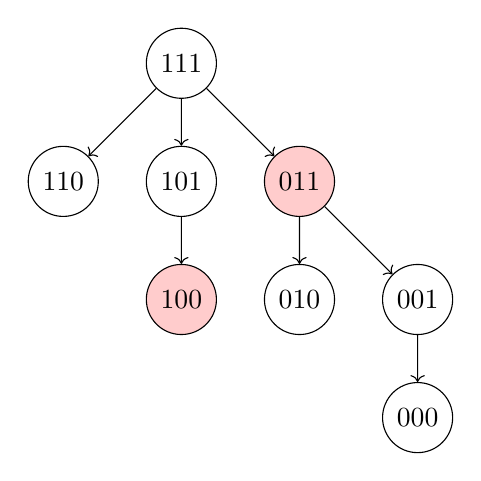
\begin{tikzpicture}[nodes={draw, circle}, ->]
        \node{111}
                child{node{110}}
                child{node {101}
                        child{ node[fill= red!20]{100} }
                }
                child{node[fill = red!20] {011}
                        child [missing]
                        child{node{010}}
                        child{node{001} 
                                child{node{000}}
                        }
                };
\end{tikzpicture}}
\caption{\label{fenwickparity} Parity set (red) for $i=6$ $(101)$ on Fenwick tree with $N=8$}
\end{figure}

\begin{figure}[htbp]
        \centerline{
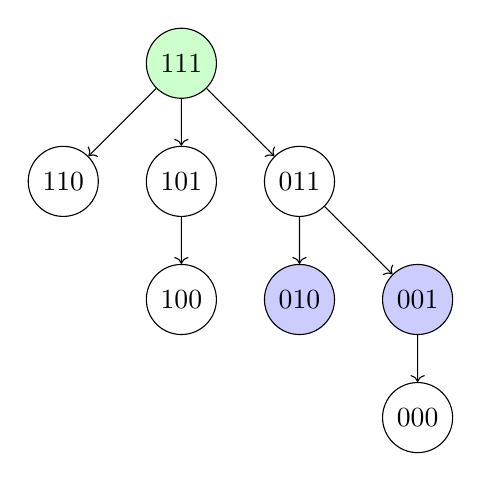
\begin{tikzpicture}[nodes={draw, circle}, ->]
        \node[fill = green!20]{111}
                child{node {110}}
                child{node {101}
                        child{ node{100} }
                }
                child{node {011}
                        child [missing]
                        child{node[fill = blue!20]{010}}
                        child{node[fill = blue!20]{001} 
                                child{node{000}}
                        }
                };
\end{tikzpicture}}
\caption{\label{fenwickupdateflip} Update set (green) and Flip set (blue) for $i=5$ $(011)$ on Fenwick tree with $N=8$}
\end{figure} \noindent
Again, the Bravyi-Kitaev operators are defined in the same way in terms of $P_i$, $U_i$ and $F_i$ as described in Section~\ref{operators}.\\\\These trees provide useful geometric intuition for considering the various sets of qubits involved in operations and for thinking about the connectivity of the mapping as discussed in Section~\ref{bravyikitavecompare}.\\\\
It is even possible to connect the Fenwick tree formulation back to the transformation matrix formulation by considering that the Fenwick trees can be constructed using an equivalent recursive process \cite{tilly}. The tree with $N = 2^n$ is built from two copies of the tree with $N = 2^{n-1}$ where all the nodes in the second tree have $2^{n-1}$ added to them and they are connected by making the root ($2^{n-1} -1$) of the first tree a child of the root ($2^n -1$) of the second tree.
\subsection{`Local' Mappings}\label{derby-klassen_section}
As physical systems are normally dominated by local interactions such as lattice hopping or Coulomb interactions, it is preferable to design a `local' mapping that has low Pauli-weights for local fermionic operators. These schemes only find representations for a selection of local interactions (usually selected to closely match the terms in the target Hamiltonian) rather than between every pair of modes like the Jordan-Wigner or Bravyi-Kitaev mapping. Generally this results in using more qubits but drastically smaller Pauli weights and thus fewer gates.\\\\ 
One strategy used to find `local' mappings is searching for sets of low weight Pauli-strings for representing the fermionic edge ($E_{jk}$) and vertex ($V_j$) operators. These are defined below in terms of the Majorana operators $\gamma_j$:
\begin{equation}
\gamma_j = a_j + a^{\dagger}_j, \> \bar{\gamma_j} = \frac{a_j - a_j^{\dagger}}{i}
\end{equation}
\begin{equation}
        E_{jk} = - i \gamma_j \gamma_k, \> V_j = - i \gamma_j \bar{\gamma_j}
\end{equation}
The full set of these operators represent the even fermionic algebra \cite{superfast} by:
\begin{equation}
        \begin{align}
                a_j^{\dagger} a_k + a_k^{\dagger} a_j &=& (\gamma_j - i \bar{\gamma_j}) (\gamma_k + i \bar{\gamma_k})  + (\gamma_k - i \bar{\gamma_k}) (\gamma_j + i \bar{\gamma_j}) &=& -\frac{i}{2}& E_{jk} (V_j - V_k)\\
                a_j^{\dagger} a_j &=& (\gamma_j - i \bar{\gamma_j}) (\gamma_j + i \bar{\gamma_j}) &=&  \frac{1}{2}& (I - V_j)\\
\end{align}
\end{equation} They are defined by their anti-commutation relations (Eq.~\ref{edgecomm}) \cite{derbyklassen} and a loop condition (Eq.~\ref{loopcond}): 
\begin{equation}
        \label{edgecomm}
        \begin{align}
                \{ E_{jk}, V_j\} = 0, \{ E_{ij}, E_{jk} \} &= 0 \> \forall \>i \neq k\\
                [V_i, V_j] =0, [E_{ij}, V_m] = 0, [E_{ij}, E_{mn}] &= 0 \>\forall \>i \neq j \neq m \neq n
\end{align}
\end{equation}
\begin{equation}
        \label{loopcond}
        i^{n} \prod_{i=1}^{n} E_{p_i p_{i+1}} = 1
        \end{equation}
        for a cyclic sequence of sites $p = \{p_1, p_2,\ldots, p_n, p_{n+1}: p_1 = p_{n+1} \}$.\\\\
       If we can find a set of Pauli-strings representing edges and vertices which satisfy these condtions then we have a mapping from even fermionic operators to qubits operators. In an intuitive sense these conditions mean:
        \begin{romanlist}
        \item Edge operators must anti-commute with any vertices they include
        \item Edge operators must anti-commute with any edges they share vertices with
        \item All vertices must commute with each other
        \item All edges that do not share a common vertex must commute
        \item All edges must commute with vertices they do not include
        \item Any cycle of edges must leave the state unchanged
        \end{romanlist}
        In a `local' mapping we find a way of mapping only a selection of these edges (ones representing local interactions) to qubit operators in such a way that the full even fermionic algebra is preserved. Charles Derby and Joel Klassen \cite{derbyklassen2} have developed a design strategy for creating representations that satisfy these restrictions for a given regular lattice of interactions. We will illustrate this technique by using the simplest case of the square lattice \cite{derbyklassen}:
                \subsubsection{Derby-Klassen mapping on square lattice}
        For a square lattice of fermionic modes, we map every vertex to a ``vertex'' qubit. Consider each square of the square lattice as either a black or white face (tiled like a chess board) and associate an additional ``face'' qubit with every black face. Let $f(i,j)$ index the unique odd face adjacent to edge $(i,j)$, and assign an orientation to the edges so they circulate clockwise or counter-clockwise around white spaces alternating every row. This is illustrated below by Fig.~\ref{squareLattice}:
\begin{figure}[htbp]
\centerline{
        \begin{tikzpicture}
                \fill [gray, opacity=0.5] (-2,2) rectangle (-1,1);
                \fill [gray, opacity=0.5] (0,2) rectangle (1,1);
                \fill [gray, opacity=0.5] (-1,1) rectangle (0,0);
                \fill [gray, opacity=0.5] (1,1) rectangle (2,0);
                \fill [gray, opacity=0.5] (-2,0) rectangle (-1,-1);
                \fill [gray, opacity=0.5] (0,0) rectangle (1,-1);
                \fill [gray, opacity=0.5] (-1,-1) rectangle (0,-2);
                \fill [gray, opacity=0.5] (1,-1) rectangle (2,-2);
                \filldraw [black] (-2,2) circle (2pt);
                \filldraw [black] (-1,2) circle (2pt);
                \filldraw [black] (0,2) circle (2pt);
                \filldraw [black] (1,2) circle (2pt);
                \filldraw [black] (2,2) circle (2pt);
                \filldraw [black] (-2,1) circle (2pt);
                \filldraw [black] (-1,1) circle (2pt);
                \filldraw [black] (0,1) circle (2pt);
                \filldraw [black] (1,1) circle (2pt);
                \filldraw [black] (2,1) circle (2pt);
                \filldraw [black] (-2,0) circle (2pt);
                \filldraw [black] (-1,0) circle (2pt);
                \filldraw [black] (0,0) circle (2pt);
                \filldraw [black] (1,0) circle (2pt);
                \filldraw [black] (2,0) circle (2pt);
                \filldraw [black] (-2,-1) circle (2pt);
                \filldraw [black] (-1,-1) circle (2pt);
                \filldraw [black] (0,-1) circle (2pt);
                \filldraw [black] (1,-1) circle (2pt);
                \filldraw [black] (2,-1) circle (2pt);
                \filldraw [black] (-2,-2) circle (2pt);
                \filldraw [black] (-1,-2) circle (2pt);
                \filldraw [black] (0,-2) circle (2pt);
                \filldraw [black] (1,-2) circle (2pt);
                \filldraw [black] (2,-2) circle (2pt);
 
                \filldraw [black] (-1.5, 1.5) circle (2pt);
                \filldraw [black] (0.5, 1.5) circle (2pt);
                \filldraw [black] (-0.5, 0.5) circle (2pt);
                \filldraw [black] (1.5, 0.5) circle (2pt);
                \filldraw [black] (-1.5, -0.5) circle (2pt);
                \filldraw [black] (0.5, -0.5) circle (2pt);
                \filldraw [black] (-0.5, -1.5) circle (2pt);
                \filldraw [black] (1.5, -1.5) circle (2pt);
                \draw [ultra thick, latex-, gray](-1.85,2) -- (-1.15,2) (2pt);
                \draw [ultra thick, latex-, gray](-0.85,2) -- (-0.15,2) (2pt);
                \draw [ultra thick, latex-, gray](0.15,2) -- (0.85,2) (2pt);
                \draw [ultra thick, latex-, gray](1.15,2) -- (1.85,2) (2pt);
                \draw [ultra thick, -latex, gray](-1.85,1) -- (-1.15,1) (2pt);
                \draw [ultra thick, -latex, gray](-0.85,1) -- (-0.15,1) (2pt);
                \draw [ultra thick, -latex, gray](0.15,1) -- (0.85,1) (2pt);
               \draw [ultra thick, -latex, gray](1.15,1) -- (1.85,1) (2pt);
               \draw [ultra thick, latex-, gray](-1.85,0) -- (-1.15,0) (2pt);
                \draw [ultra thick, latex-, gray](-0.85,0) -- (-0.15,0) (2pt);
                \draw [ultra thick, latex-, gray](0.15,0) -- (0.85,0) (2pt);
                \draw [ultra thick, latex-, gray](1.15,0) -- (1.85,0) (2pt);
                \draw [ultra thick, -latex, gray](-1.85,-1) -- (-1.15,-1) (2pt);
                \draw [ultra thick, -latex, gray](-0.85,-1) -- (-0.15,-1) (2pt);
                \draw [ultra thick, -latex, gray](0.15,-1) -- (0.85,-1) (2pt);
               \draw [ultra thick, -latex, gray](1.15,-1) -- (1.85,-1) (2pt);
               \draw [ultra thick, latex-, gray](-1.85,-2) -- (-1.15,-2) (2pt);
                \draw [ultra thick, latex-, gray](-0.85,-2) -- (-0.15,-2) (2pt);
                \draw [ultra thick, latex-, gray](0.15,-2) -- (0.85,-2) (2pt);
                \draw [ultra thick, latex-, gray](1.15,-2) -- (1.85,-2) (2pt);

                \draw [ultra thick, -latex, gray](2,-1.85) -- (2,-1.15) (2pt);
                \draw [ultra thick, -latex, gray](2,-0.85) -- (2,-0.15) (2pt);
                \draw [ultra thick, -latex, gray](2,0.15) -- (2,0.85) (2pt);
                \draw [ultra thick, -latex, gray](2,1.15) -- (2,1.85) (2pt);
                \draw [ultra thick, latex-, gray](1,-1.85) -- (1,-1.15) (2pt);
                \draw [ultra thick, latex-, gray](1,-0.85) -- (1,-0.15) (2pt);
                \draw [ultra thick, latex-, gray](1,0.15) -- (1,0.85) (2pt);
               \draw [ultra thick, latex-, gray](1,1.15) -- (1,1.85) (2pt);
               \draw [ultra thick, -latex, gray](0,-1.85) -- (0,-1.15) (2pt);
                \draw [ultra thick, -latex, gray](0,-0.85) -- (0,-0.15) (2pt);
                \draw [ultra thick, -latex, gray](0,0.15) -- (0,0.85) (2pt);
                \draw [ultra thick, -latex, gray](0,1.15) -- (0,1.85) (2pt);
                \draw [ultra thick, latex-, gray](-1,-1.85) -- (-1,-1.15) (2pt);
                \draw [ultra thick, latex-, gray](-1,-0.85) -- (-1,-0.15) (2pt);
                \draw [ultra thick, latex-, gray](-1,0.15) -- (-1,0.85) (2pt);
               \draw [ultra thick, latex-, gray](-1,1.15) -- (-1,1.85) (2pt);
               \draw [ultra thick, -latex, gray](-2,-1.85) -- (-2,-1.15) (2pt);
                \draw [ultra thick, -latex, gray](-2, -0.85) -- (-2,-0.15) (2pt);
                \draw [ultra thick, -latex, gray](-2, 0.15) -- (-2,0.85) (2pt);
                \draw [ultra thick, -latex, gray](-2, 1.15) -- (-2,1.85) (2pt);
                \node[below] at (-1.5,1.5) {\small $f(i,j)$};
                \node[below right] at (-1,2) {\small $i$};
                \node[above right] at (-1,1) {\small $j$};
        \end{tikzpicture}
}

\fcaption{\label{squareLattice} A square lattice of black and white faces with a face qubit assigned to every black face illustrating how edges are assigned orientation}
\end{figure}
The design strategy involves mapping each edge operation to a Pauli string acting with a Y gate acting on the qubit at the head of the arrow and an X gate acting on the qubit at the tail of the arrow, and each vertex operation to a Z gate acting on the vertex. This is illustrated in Fig~\ref{derbyklassenline}:\\
\begin{figure}[htbp]
\centerline{
        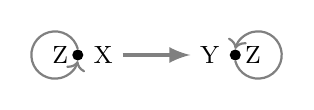
\begin{tikzpicture}
                \node[circle, fill, minimum size =4, inner sep = 0, label={[name=left]right:{\small X}}](L) at (-1,0) {};
                \node[circle, fill, minimum size =4, inner sep = 0, label={[name=right]left:\small Y}](R) at (1,0) {};
\draw[ultra thick, -latex, gray] (left.east) --  (right.west);
\draw [thick, ->, gray] (L.north)arc(15:345:0.3);
                                    \node[left, black] at (L) {\small Z};
                                    \draw [thick, ->, gray] (R.south)arc(-165:165:0.3);
                                    \node[right, black] at (R) {\small Z};

        \end{tikzpicture}}
        \fcaption{\label{derbyklassenline} Illustration of how an edge operator and two vertex operators act on adjacent qubits}
\end{figure}\\
Straight away this can be seen to satisfy the intuitive conditions i), iii), iv) and v). Also as $X$ and $Y$ anti-commute, it is clear that every pair of edges that meet head-to-tail anti-commute, whereas pairs of edges that meet head-to-head or tail-to-tail commute. We can correct this behaviour by mapping every pair of these edges, those which currently commute but should anti-commute, to act upon a common ancillary qubit with X and Y gates respectively. Though this procedure is performed on a directed graph it still holds for edges in both directions as $E_{ij} = -E_{ji}$, so if $E_{ij}$ anti-commutes with an operator so will $E_{ji}$. Therefore, by adding ancillary qubits we can make the mapping also satisfy restriction ii).
\\\\ On a square lattice this common ancillary qubit can be the face qubit adjacent to the edges, as every pair of head-to-head or tail-to-tail edges share a common face qubit (see Fig~\ref{squareLattice}). It can be seen that using an ancillary ``face'' qubit to introduce two separate anti-commutation relations does not break the restriction iv), as long as opposite edges of black squares act in commutable ways upon the ``face'' qubit (i.e. with same gate). \\\\
In order to satisfy the loop condition, applying any given loop of edges needs to correspond to an identity in the fermionic Fock space. This is achieved by mapping from the even fermionic algebra to the Pauli operator code space stabilised by the representation of cycles of edges. Therefore, all sets of Pauli strings produced by this mapping must commute with the stabilisers generated by each cycle of edges. Below we consider conditions upon these stabilisers such that the representation of the even fermionic algebra in Pauli operators is non-trivial (this treatment is adapted from \cite{derbyklassen2}):
\begin{romanlist}
\item Let $M_G$ be the group of directed edges $e_{ij}$ and vertices $v_{i}$ which satisfy Eq.~\ref{edgecomm} for a given graph $G$, and $C_G$ be the directed cycles of graph $G$
\item First, we show that every operation in the full even fermionic algebra ($M_E$) represented in terms of $E_{ij}$ and $V_j$ can be one-to-one mapped to a composition of cosets of the cycles ($e_{ij}C_G$ and $v_iC_G$) of an arbitrary spanning connected subgraph ($M_G/C_G$).
        \begin{alphlist}
        \item Define the following invertible transformation for all edges and vertices in $G$:
                \begin{equation}
                        \begin{align}
                                M_G/C_G &\longleftrightarrow M_E\\
                                v_i C_G &\longleftrightarrow V_i\\
                         e_{ij}C_G &\longleftrightarrow E_{ij}
                        \end{align}
                \end{equation}
        \item $M_E$ contains all the possible edges not just those in $G$. As $G$ is connected, all edges not in $G$ can be constructed by composition of defined edge operators in $G$. Define this composition as:
                \begin{equation}
                        e_{ik} = e_{ij} \circ e_{jk} \longleftrightarrow E_{ik} = i E_{ij} E_{jk}
                \end{equation}
        \item As $M_G$ satisfies Eq.~\ref{edgecomm} for all $e_{ij}$ and $v_i$ in $G$, this holds for $M_G/C_G$, and therefore for all $E_{ij}$ and $V_{i}$ in $G$.
        \item All $E_{ij}$ not in $G$ can be decomposed into $E_{ij}$ in $G$ and the introduced phase difference will have no impact on Eq.~\ref{edgecomm}. Therefore, all edges and vertices satisfy the anti-commutation and commutation relations
        \item All cyclic paths in $G$ satisfy Eq.~\ref{loopcond} as:
                \begin{equation}
                       I = f(IC_G) = f\left( i^{n} \prod_{i=1}^n e_{p_i, p_{i+1}} C_G \right) =  i^{n} \prod_{i=1}^n E_{p_i, p_{i+1}}
                \end{equation}
                \item All cyclic paths that include edges ($\tilde E_{ij}$) not in $G$ also satisfy Eq.~\ref{loopcond} as the definition of composition adds a factor of $i$ for every edge that gets added so the total phase is preserved:
                \begin{multline}
                        i^{n+2} \prod^n_{i=0}E_{p_i,p_{i+1}} \tilde E_{p_{n-1}, p_n} \tilde E_{p_n p_{n+1}} =\\ i^{n+2} \prod^n_{i=0}E_{p_i,p_{i+1}} i E_{p_{n-1}, p_k} E_{p_k, p_{n}} i E_{p_{n}, p_l} E_{p_l, p_{n+1}}= i^{n+4} \prod^{n+4}_{i=1}E_{p_i, p_{i+1}} = I
                \end{multline}
        \end{alphlist} $\square$.
\item Next, we prove that this quotient group $M_G/C_G$ has a faithful representation in Pauli operators, if there exists a representation of $M_G$ with a stabiliser containing $C_G$ which in turn has a non-trivial codespace ($+1$ common eigenspace):
        \begin{alphlist}
        \item The group $M_G$ has a representation $\sigma$ in the Hilbert space $\mathcal{H}$ of a system of qubits
        \item If a stabiliser of a non-trival subgroup of $\sigma$ contains all the elements of $C_G$, then can define new representation $\tau$ as:
                \begin{equation}
                        \tau (m C_G) = Proj_U \circ \sigma(m) \> \forall \> m \in M_G/C_G
                \end{equation}
                with $U$ the common +1 eigenspace of $\sigma(C_G)$.
        \end{alphlist}
\item Recall, that if $\sigma$ is a representation in the multi-qubit Pauli operators $\{\pm 1, \pm i\} \times^N_i \{I_i, X_i, Y_i, Z_i\}$ then any subgroup $S$ that is abelian and does not contain $-I$ is the stabiliser of a non-trivial vector space \cite{nielsenChuang}.
\item Finally we find a stabiliser of the representation of $M_G$ containing $C_G$ using iv). As $C_G$ is abelian \cite{derbyklassen2}, $\sigma(C_G)$ is abelian. Therefore, if $-I\>\> \cancel \in \>\>\sigma(C_G)$, then $\sigma(C_G)$ is a stabiliser of $\sigma$ with a non-trivial $+1$ common eigenspace (codespace).
\item Therefore, $M_G/C_G$ (and hence $M_E$) has a faithful representation $\tau$ in Pauli operators, in particular in the code space of $\sigma(C_G)$
\end{romanlist}
Therefore, the mapping we have found is valid as long as no cycle is mapped to $-I$. As all cycles on this square lattice can be decomposed into a combination of cycles around single black and white faces \cite{derbyklassen2}, we only need to consider these stabiliser generators individually. \\\\
As shown in Fig~\ref{blackfaceloops}, looping a black face produces $-I$ meaning it cannot be in a stabilizer, however this can be fixed by simply flipping the sign of one of the four edges. Then we get $X_1Y_5Y_2 \otimes -Y_2X_5X_3 \otimes X_3Y_5Y_4 \otimes Y_4 X_5 X_1 = -X_1^2 Y_2^2 X_3^2 Y_4^2 (Y_5X_5)^2 = - (iZ_5)^2 = I$.
\begin{figure}[htbp]
\centerline{
        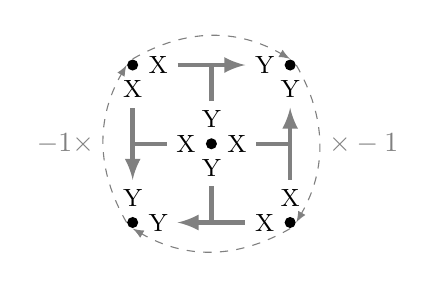
\begin{tikzpicture}
                \node[circle, fill, minimum size =4, inner sep = 0, label={[name=bottomLeftY]right:{\small Y}}, label={[name=bottomLeftY2]above:{\small Y}}](BL) at (-1,-1) {};
                \node[circle, fill, minimum size =4, inner sep = 0, label={[name=topLeftX]below:\small X}, label={[name=topLeftX2]right:\small X}](TL) at (-1,1) {};
                \node[circle, fill, minimum size =4, inner sep = 0, label={[name=bottomrightX]left:\small X},  label={[name=bottomrightX2]above:\small X}](BR) at (1,-1) {};
                \node[circle, fill, minimum size =4, inner sep = 0, label={[name=toprightY]left:\small Y}, label={[name=toprightY2]below:\small Y}](TR) at (1,1) {};
                \node[circle, fill, minimum size =4, inner sep = 0, label={[name=centreX1]left:\small X}, label={[name=centreX2]right:\small X},label={[name=centreY1]below:\small Y}, label={[name=centreY2]above:\small Y}] at (0,0) {};

                                \draw[ultra thick, latex-, gray] (bottomLeftY.east) -- node [midway](BL2BR){} (bottomrightX.west);
                                
                                \draw[ultra thick, -, gray] (centreY1.south) -- (BL2BR.center);
                                \draw[ultra thick, latex-, gray] (bottomLeftY2.north) --  node [midway](BL2TL){} (topLeftX.south);
                                \draw[ultra thick, -latex, gray] (topLeftX2.east) --  node [midway](TL2TR){} (toprightY.west);
                                \draw[ultra thick, -latex, gray] (bottomrightX2.north) --  node [midway](BR2TR){} (toprightY2.south);
                                 \draw[ultra thick, -, gray] (centreY2.north) -- (TL2TR.center);

                                  \draw[ultra thick, -, gray] (centreX1.west) -- (BL2TL.center);

                                   \draw[ultra thick, -, gray] (centreX2.east) -- (BR2TR.center);
                                   \draw[dashed,-latex, gray ] (BL.west)  to[bend left] node[left] {$-1 \times$}  (TL.west);
                                   \draw[dashed,-latex, gray] (BR.south) to[bend left](BL.south);
                                   \draw[dashed,-latex, gray] (TL.north) to[bend left](TR.north);
                                   \draw[dashed,-latex, gray] (TR.east) to[bend left] node[right] {$\times -1$} (BR.east) ;


                   \end{tikzpicture}}
           \fcaption{\label{blackfaceloops} Diagram of looping around black face. This gives $X^2 = Y^2 = I$ at every ``vertex'' qubit, but $(-X)Y(-X)Y = (XY)^2 = (iZ)^2 = -I$ at the ``face'' qubit, so overall $-I_5I_1I_2I_3I_4 = -I$. The two negative signs introduced by having to flip the orientation of the vertical edges cancel each other out.}
   \end{figure}\\
   It can be seen in Fig~\ref{whitefaceloops}, that looping a white face produces a non-trivial stabilizer, which is not $-I$. Therefore, using the mapping described (with the sign flipped on one edge of every black face) will give a faithful representation of the even fermionic algebra. All valid even fermionic operations will be mapped into the code space of the stabilizers around white faces, meaning the Pauli string representations will commute with every element of this stabilizer group. \\
\begin{figure}[htbp]
\centerline{
        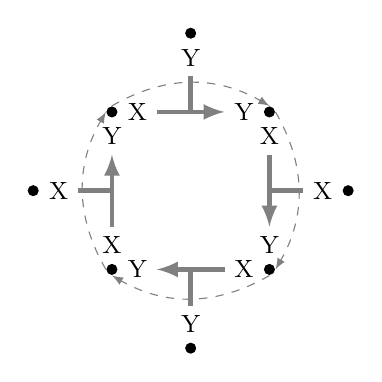
\begin{tikzpicture}
                \node[circle, fill, minimum size =4, inner sep = 0, label={[name=bottomLeftY]right:{\small Y}}, label={[name=bottomLeftY2]above:{\small X}}](BL) at (-1,-1) {};
                \node[circle, fill, minimum size =4, inner sep = 0, label={[name=topLeftX]below:\small Y}, label={[name=topLeftX2]right:\small X}](TL) at (-1,1) {};
                \node[circle, fill, minimum size =4, inner sep = 0, label={[name=bottomrightX]left:\small X},  label={[name=bottomrightX2]above:\small Y}](BR) at (1,-1) {};
                \node[circle, fill, minimum size =4, inner sep = 0, label={[name=toprightY]left:\small Y}, label={[name=toprightY2]below:\small X}](TR) at (1,1) {};
                \node[circle, fill, minimum size =4, inner sep = 0, label={[name=centreX1]right:\small X}] at (-2,0) {};
                \node[circle, fill, minimum size =4, inner sep = 0, label={[name=centreX2]left:\small X}] at (2,0) {};
\node[circle, fill, minimum size =4, inner sep = 0, label={[name=centreY2]below:\small Y}] at (0,2) {};
\node[circle, fill, minimum size =4, inner sep = 0, label={[name=centreY1]above:\small Y}] at (0,-2) {};

                                \draw[ultra thick, latex-, gray] (bottomLeftY.east) -- node [midway](BL2BR){} (bottomrightX.west);
                                
                                \draw[ultra thick, -, gray] (centreY1.north) -- (BL2BR.center);
                                \draw[ultra thick, -latex, gray] (bottomLeftY2.north) --  node [midway](BL2TL){} (topLeftX.south);
                                \draw[ultra thick, -latex, gray] (topLeftX2.east) --  node [midway](TL2TR){} (toprightY.west);
                                \draw[ultra thick, latex-, gray] (bottomrightX2.north) --  node [midway](BR2TR){} (toprightY2.south);
                                 \draw[ultra thick, -, gray] (centreY2.south) -- (TL2TR.center);

                                  \draw[ultra thick, -, gray] (centreX1.east) -- (BL2TL.center);

                                   \draw[ultra thick, -, gray] (centreX2.west) -- (BR2TR.center);
                                   \draw[dashed,-latex, gray ] (BL.west)  to[bend left]  (TL.west);
                                   \draw[dashed,-latex, gray] (BR.south) to[bend left](BL.south);
                                   \draw[dashed,-latex, gray] (TL.north) to[bend left](TR.north);
                                   \draw[dashed,-latex, gray] (TR.east) to[bend left] (BR.east) ;


                   \end{tikzpicture}}
                   \fcaption{\label{whitefaceloops} Diagram of stabiliser given by looping around a white face}
   \end{figure}\\
Therefore, we can map the edges in the direction of their assigned orientation as:
\begin{equation}
                E_{ij} = \begin{cases}
                        X_i Y_j X_{f(i,j)} & (i,j) \text{ oriented downwards}\\
                        -X_i Y_j X_{f(i,j)} & (i,j) \text{ oriented upwards}\\
                        X_i Y_j Y_{f(i,j)} & (i,j) \text{ horizontal}\\
                \end{cases}
        \end{equation}
        with the last term ignored if the edge lies on a boundary with no adjacent face qubit. Traversing edges in the opposite direction to their orientation just involves applying a sign change. \\\\We also map the vertex operators to:
        \begin{equation}
                V_j = Z_j
        \end{equation}
        This gives a map from pauli strings to edges and vertices which in turn form a representation of the even fermionic algebra. For instance, 
        \begin{equation}
               H =  a_1 a_2^{\dagger} + a_1^{\dagger} a_2 \longleftrightarrow - \frac{i}{2} E_{12} (V_1 - V_2) \longleftrightarrow -\frac{i}{2}X_1 Y_2 Y_{f(1,2)}( Z_1 -Z_2)
        \end{equation}
        where $(1,2)$ is taken to be horizontal. The stabiliser group formed by Fig~\ref{whitefaceloops} on every white square would act with $Y_{f(1,2)}Z_1Z_2$, $X_{f(1,2)}Z_1$ or $X_{f(1,2)} Z_2$ on the qubits at hand. These clearly commute with the operation:
        \begin{multline}
        (Y_{f(1,2)} Z_1 Z_2) (-\frac{i}{2}X_1 Y_2 Y_{f(1,2)}( Z_1 -Z_2))
        = - \frac{i}{2} Z_1 X_1 Z_2 Y_2 (Z_1 - Z_2) Y_{f(1,2)}^2 \\= - \frac{i}{2} (- X_1 Z_1) (- Y_2 Z_2) ( Z_1 - Z_2) Y_{f(1,2)}^2 = - \frac{i}{2} X_1 Y_2 Y_{f(1,2)} (Z_1 - Z_2) Z_1 Z_2 Y_{f(1,2)} 
\end{multline}
\begin{multline}
        (X_{f(1,2)} Z_1 ) (-\frac{i}{2}X_1 Y_2 Y_{f(1,2)}( Z_1 -Z_2))
        = - \frac{i}{2} Z_1 X_1 Y_2 (Z_1 - Z_2) X_{f(1,2)}Y_{f(1,2)} \\= - \frac{i}{2} (- X_1 Z_1)  Y_2  ( Z_1 - Z_2) (-  Y_{f(1,2)}X_{f(1,2)} )= - \frac{i}{2} X_1 Y_2 Y_{f(1,2)} (Z_1 - Z_2) X_{f(1,2)} Z_1 \end{multline}
Therefore, the operation lies in the code space of the stabiliser group as expected.\\\\
        The above only defines a mapping for the even (not the full) fermionic algebra, however, as all physical fermionic operators preserve parity this represents all physical fermionic operators. It is also possible to extend this mapping on some lattice sizes to the full fermionic algebra by injecting Majorana operators at the corners, however, this is not discussed here (this treatment can be found in \cite{derbyklassen} and \cite{derbyklassen2}).\\\\
The Derby-Klassen design scheme can be applied broadly to a number of regular lattices by following the above principle of assigning orientations to edges and using shared ancilla qubits to resolve head-to-head or end-to-end anti-commutation relations. So far applications have been found to all uniform tilings of degree less than 4 and cubic lattices.\\\\
The Derby-Klassen mapping is just one example of many 'local' mappings which use ancillia qubits to produce constant Pauli weight interaction terms. It was the most efficient local mapping in the literature as it only requires 1.5 qubits per fermionic mode, compared to the 2 of Verstraete-Cirac, exact bosonization and Bravyi-Kitaev superfast mappings. However, recently published research by Chen and Xu \cite{chenxu} describes a super-compact mapping only requiring 1.25 qubits per fermionic mode. The super-compact mapping has a higher constant average Pauli weight, however, in the NISQ era with limited qubits available this is a negligible consideration compared to the reduction in ancilla qubits needed. Chen and Xu \cite{chenxu} also showed that every existing `local' mapping can be derived from applying generalised local unitary circuits to the exact bosonization map described in \cite{chen2}.
                  \section{Relative performance of mappings}\label{comparision_section}
                  Each of these encodings offers various advantages and disadvantages when applied to real applications such as VQEs or phase estimation discussed in Section~\ref{applications_section}. As explained in Section~\ref{vqe_section}, the efficency of these techniques is broadly based on three factors: number of qubits required, average Pauli-weight and the number of distinct Pauli-strings in the Hamiltonian. When applied to Quantum Phase Estimation there is the additional consideration of Trotter error as described in Section~\ref{trotter}. All of the different mappings make different trade-offs between these factors.\\\\
   There are some techniques \cite{reducequbits} which decrease the number of qubits required by increasing the number of distinct Pauli-strings, however we have not covered them here. All the techniques discussed in this essay leave the number of terms in the Hamiltonian unchanged.\\\\
   In this section, comparisions are drawn between the different mappings. First, the relative advantage of `local' mappings and `non-local' mappings are considered in Section~\ref{local1}. Then, in Section~\ref{bravyikitavecompare} a comparison between the Bravyi-Kitaev and Jordan-Wigner mapping is considered in the context of Quantum Phase Estimation. Classical simulations of QPE feature heavily in Section~\ref{bravyikitavecompare}.
           \subsection{'Local' versus 'non-local' mappings}\label{local1}
The main trade-off at play is between the Jordan-Wigner/Bravyi-Kitaev style mappings and the 'local' (Derby-Klassen style) mappings. 'Local' mappings sacrifice an increased qubit count for drastically more localised operations. Applying a local fermionic interaction on a Jordan-Wigner or Bravyi-Kitaev mapping will take $O(N)$ and $O(\log(N))$ gates respectively, whereas on the Derby-Klassen square lattice mapping it only takes 3. This significant reduction in gate count is coupled with an increase in qubit count with Derby-Klassen requiring 1.5 qubits per fermionic mode compared to the 1 qubit per mode that Jordan-Wigner and Bravyi-Kitaev need. However, the constant gate count only holds for local interactions and performing an operation involving two arbitrary modes would scale with the diameter of the graph of local interactions. Therefore, the Derby-Klassen design scheme is only useful for Hamiltonians with local interactions, and is most effective for interactions on a regular lattice for which a mapping is known \cite{derbyklassen2}. These include all uniform tilings of degree less than 4, and the cubic lattice. 
\subsection{Bravyi-Kitaev mapping versus Jordan-Wigner mapping for QPE}\label{bravyikitavecompare}
There is also an important discussion to be had about the relative merits of the Jordan-Wigner and Bravyi-Kitaev transformations. As we have discussed Bravyi-Kitaev has theoretically logarithmically superior scaling in Pauli-weights, however the experimental simulations show a more nuanced picture. It has been shown that Bravyi-Kitaev leads to a small reduction in the number of gates needed to simulate molecular Hydrogen in a minimal basis \cite{seeley}. However, for larger chemicals where we would expect the scaling advantage to grow the results are more muddled.\\\\
Tranter et al. \cite{tranter2018} preformed classical simulations of quantum phase estimation on 86 molecular systems using the Bravyi-Kitaev and Jordan-Wigner mappings. They found that with no optimisation and magnitude Trotter-ordering the Bravyi-Kitaev mapping showed a consistent improvement of up to 25\% shorter circuits, but only for molecules with more than roughly 30 spin-orbitals. This reflects the additional overhead required to implement Bravyi-Kitaev, as gates must be applied to at most $4 \log(N)+2$ qubits for every even fermionic operation (if $U(i)$, $U(j)$, $R_i$ and $R_j$ are disjoint), rather than at most $N$ qubits for Jordan-Wigner. This gives Bravyi-Kitaevv a larger prefactor and makes Jordan-Wigner more efficient for small systems. When gate optimisation (e.g. removing duplicate gates)  was introduced the Bravyi-Kitaev mapping pulled even further ahead with roughly 30-40\% shorter circuits. It is worth noting that another significant advantage of the Bravyi-Kitaev mapping is a large reduction in the number of entangling CNOT gates in exchange for a small up-tick in single qubit gates. This could make the mapping easier to implement on near-term experimental devices, as it is harder to implement 2-qubit gates.
\fnt{b}{A lexicographic ordering is essentially an alphabetic ordering with respect to the Pauli strings that make up each Hamiltonian term. This attempts to maximise cancellation of CNOT gates by changing the least number of qubits between terms. From Fig~\ref{trotterStepCircuit} it can be seen how concatenating a circuit with only the fourth qubit changed would led to two CNOTs, an $R_X^{\dagger}$ and Hadamard gate cancelling out (as $H^2 = CNOT^2 = R_X^{\dagger}R_X = I$).}
\\\\Additionally, they showed that a large amount of the advantage afforded by Bravyi-Kitaev over Jordan-Wigner is eliminated through the use of a better Trotter-ordering. Using an optimised lexicographic\fnm{b} ordering the mappings appear equivalent for small molecules, and for some larger molecules Jordan-Wigner resulted in marginally shorter circuits and lower CNOT counts. They attributed this to the complexity of the Bravyi-Kitaev mapping reducing the linearity of the CNOT chains and so being less optimisable. It should be emphasised that the lexicographic ordering drastically reduced circuit lengths for all mappings, so the better ordering simply had more of an impact upon the Jordan-Wigner mapping rather than increasing the circuit length of the Bravyi-Kitaev mapping. This behaviour was only shown to hold for lexicographic ordering, so it is unclear how an optimum ordering in Bravyi-Kitaev would perform against an optimum ordering in Jordan-Wigner.\\\\
Tranter et al. \cite{tranter2018} also investigated the impact of the two different mappings upon the Trotter error. However, the results were limited as determining the Trotter error is a hard problem owing to the difficulty in finding the exact ground state energy for use as a reference point. Therefore, they were only able to consider small systems where they found that with lexicographic encoding the Trotter error was lower (in some cases half) for Bravyi-Kitaev compared with Jordan-Wigner. However, for these systems the error was so small it would make a neglible impact compared to the difference in circuit length of individual Trotter steps discussed above. It was hypothesied that if this reduction in error also holds for larger systems then it may significantly reduce the number of Trotter steps necessary to achieve a desired accuracy. So it is possible that in the case of lexicographic ordering the reduction in Trotter steps due to the lower errors of Bravyi-Kitaev may outweigh the small increase in circuit length making it the preferable choice. However, further research is needed to determine the impact of different mappings on the Trotter error for large systems so we can draw no definite statements.\\\\
One consideration which was not explored by Tranter et al., is the differing qubit connectivity required by the two schemes as discussed in \cite{codes}. In real world architecture, qubits have to be physically laid out and not every qubit is connected to every other. This means often only adjacent pairs of qubits have physical 2-qubit gates between then, therefore to entangle distant qubits requires multiple real 2-qubit gates to produce one virtual 2-qubit gate. Both the mappings transform fermionic Hamiltonians into a series of Pauli strings, and when performing phase estimation the exponentials of these Pauli strings must be simulated. As shown in Fig~\ref{trotterStepCircuit}, exponentiating a Pauli string requires applying CNOT gates between every consecutive qubit involved. Therefore, the more accurately the Pauli strings generated by the mappings match the connectivity of qubit architecture the fewer additional 2-qubit gates will be required. This will depend upon each individual quantum device, but we will only consider the simple case of a square lattice architecture. Here the Jordan-Wigner map can be easily mapped on to a square lattice using for example an S-pattern embedding. Every Pauli string in this embedding would lie along the connectivity graph, therefore requiring no additional 2-qubit gates. On the other hand, the Bravyi-Kitaev is harder to embed as it generates Pauli strings that navigate a fenwick tree structure. In fact once the number of modes exceeds 16 it becomes impossible to embed the tree into a square lattice without mapping neighbouring modes in the tree to non-adjacent qubits \cite{codes}, thus requiring additional 2-qubit gates. This increasingly complex connectivity puts the Bravyi-Kitaev mapping at a distinct disadvantage, as the marginal improvements in circuit size described above will quickly become negligible compared to the extra CNOT gates required to entangle non-adjacent qubits.\\\\
Finally, there is some evidence \cite{noiseerror} that the Bravyi-Kitaev mapping is more susceptible to noise-induced errors than the Jordan-Wigner mapping (for UCC ansatz preparation \cite{tilly} when simulating ground state energies of small diatomic molecules). This is surprising as the Bravyi-Kitaev mapping resulted in fewer gates on average (in these trials), so one would expect less noise-induced error. It was hypothesised this result was because a single qubit flip in the Jordan-Wigner mapping only affects one occupation number, whereas in the Bravyi-Kitaev mapping it would affect several. However, further study is needed to test this hypothesis, and to detemine which mapping is more robust to noise for larger problem sizes.\\\\
In conclusion, when given the choice between these two mappings to perform a Quantum Phase Estimation, if the qubit architecture allows all-to-all connectivity then the Bravyi-Kitaev mapping seems the most appropriate choice. For all optimisations or orderings the Bravyi-Kitaev mapping significantly outperformed the Jordan-Wigner transformation, with the exception of optimised lexicographic ordering when it was comparable. Despite optimised lexicographic ordering giving the optimal gate count reduction it may be suboptimal for minimising the Trotter error, so an ordering with a clear advantage for the Bravyi-Kitaev mapping might be used instead. However, in the NISQ era qubit architecture will often be more restricted. Therefore, the optimal choice on current devices is the Jordan-Wigner transformation as it provides comparable performance (when using lexicographic ordering) with much simpler connectivity.
               \section{Fermionic Enumeration}\label{fermionic-enumeration_section}
               Mitchell Chiew and Sergii Strelchuk \cite{fermionicEncoding} realised that for the Jordan-Wigner mapping there is the potential for reducing resource costs without changing anything other than the order we encode qubits. This is achieved by improving the locality of the mapping, so local operations have lower Pauli weights. The following treatment is adapted from \cite{fermionicEncoding}: \\\\
               In 1-D the enumeration is trivial, however, in 2D it becomes an interesting problem. For instance, consider a fermionic square lattice every mode must be assigned a qubit from a 1-D qubit array. There are many different ways of accomplishing this; most notably the S or Z pattern illustrated in Fig~\ref{SZpattern}. As discussed in Section~\ref{derby-klassen_section}, we are often interested in Hamiltonians with local interactions (e.g. between adjacent modes in the lattice). Therefore, the particular enumeration you use will impact the number of qubits that lie between neighbouring modes in the lattice. This is important as in the Jordan-Wigner transformation the Pauli-weight of a fermionic operation scales with the difference in enumeration. Thus by minimising the difference in enumeration between adjacent modes we minimise the average Pauli-weight of local interactions. This reduces to the problem of simple optimal linear arrangement (or edgesum) \cite{edgesum} from graph theory, and is formulated as:\\\\
               \textbf{Simple Optimal Linear Arrangement}: For a graph G with vertices V and edges E. Find an enumeration scheme $f: V \rightarrow \{1,2,...,n\}$ that minimises the cost function
               \begin{equation}
                       C(f) = \sum_{\alpha, \beta} |f(\alpha) - f(\beta)| \label{SOLA}
               \end{equation}
               where the average Pauli weight is given by $\frac{C(f)}{|E|} +1$.\\\\
               This problem is NP-complete \cite{edgesum} though a number of solutions are known for a range of graphs. We will consider the case of the square lattice to illustrate the principle, but it could be equally well applied to any of the other graphs with known solutions.
               \begin{figure}[htbp]
                       \centerline{
                       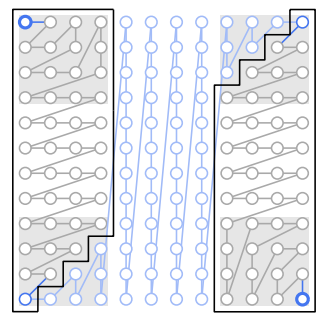
\includegraphics[scale=0.65]{mitchison-durbin.png}
               }
               \caption{\label{mitchisondurbin} The Mitchison-Durbin pattern with regions $U$ and $V$ outlined (taken from \cite{fermionicEncoding})}
               \end{figure} \\\\
               The Mitchison-Durbin pattern (illustrated in Fig~\ref{mitchisondurbin}) provides the fermion enumeration scheme that minimises the average Pauli weight of hopping terms in a square lattice. Below we present a brief summary of the proof of this (found in \cite{fermionicEncoding} and \cite{mitchisondurbin}):
               \begin{itemlist}
               \item \textbf{Lemma 7.1}: The minimum  cost will be attained by a horizontally and vertically ordered enumeration (numbering increases from left to right and from top to bottom)
                        \begin{alphlist}
                        \item It can be shown that horizontal ordering never increases the vertical contributions, and clearly always decreases the horizontal ordering
                        \item Similarly, vertical ordering can be shown to never increase the cost
                        \item It can be proven that vertical ordering preserves horizontal ordering and vice verse
                        \item Therefore, given an optimal enumeration we can apply horizontal and vertical ordering together without increasing the cost, so the minimum cost will be attained by a horizontally and vertically ordered enumeration
                                      \end{alphlist}
       \item \textbf{Lemma 7.2}: Given a horizontally and vertically ordered enumeration scheme for the lattice, the cost function for the minimum-1-sum problem is:
               \begin{equation}
                       C(f) = \sum_{\alpha\in V_b} f(\alpha) + \sum_{\alpha\in V_r} f(\alpha) - \sum_{\alpha\in V_l} f(\alpha) - \sum_{\alpha\in V_t} f(\alpha) \label{hvSOLA}
               \end{equation}
               where $V_b$, $V_r$, $V_l$ and $V_t$ are the vertices in the bottom row, right column, left column and top row respectively.\\\\
               \textbf{Proof}: As horizontally and vertically ordered every absolute sign in Eq.~\ref{SOLA} can be evaluated:
                       \begin{equation}
                               C(f) = \sum_{(\mu, \nu) \in V} f(\mu+1, \nu) - f(\mu, \nu) + f(\mu, \nu+1) - f(\mu, \nu)
                       \end{equation}
                       \begin{equation}
                       C(f) = \sum_{(\mu, \nu) \in V} f(\mu+1, \nu) - f(\mu, \nu) + \sum_{(\mu,\nu) \in V} f(\mu, \nu+1) - f(\mu, \nu)
                               \end{equation}
                               \begin{equation}
                                       C(f) = \sum_{\nu = 1}^N f(N, \nu) - f(1, \nu) + \sum_{\mu =1}^1 f(\mu, N) - f(\mu, 1)
                               \end{equation}
                               \begin{equation}
                       C(f) = \sum_{\alpha\in V_r} f(\alpha) - \sum_{\alpha\in V_l} f(\alpha) + \sum_{\alpha\in V_b} f(\alpha) - \sum_{\alpha\in V_t} f(\alpha) 
               \end{equation}
               $\square.$
       \item The Mitchison-Durbin mapping splits the lattice into three regions $U$, $V$ and $\bar U \cup \bar V$, with $U$ initially the section containing labels up to $(N,1)$ and $V$ initially containing labels from $(1,N)$. These two regions form upper- and lower- skew block-triangular sections in a vertical and horizontally ordered enumeration. The first step taken is to maximise the sum $S(U)$ of labels on the boundary of the lattice in $U$ and minimise the same sum $S(V)$ in $V$, in order to minimise $C(f)$ given by Eq.~\ref{hvSOLA}. The rules for maximising $S(U)$ are:
               \begin{alphlist}
               \item Start with the top left vertex, and start numbering by moving along every new row or column as far as horizontal and vertical ordering allows. As if the row or column is not filled maximally, then the next column or row to be filled will start with a lower enumeration, decreasing $S(U)$.
               \item Then move to the longest remaining column or row starting with the top-leftmost available vertex of the lattice. As given two columns or rows of length $b > a$ and initial enumeration $i$, filling $b$ first gives contribution $i + (i+b)$ to $C(f)$ whereas filling $a$ first gives a contribution $i + (i+a)$.
               \end{alphlist}
               By symmetry, the reverse of this process minimises $S(V)$. The final region $\bar U \cup \bar V$ should be filled with columns to maximise the labels of the top row and minimise the labels of the bottom row. This uniquely determines the minimum cost enumeration for given $U$ and $V$.
       \item It can be shown $U$ and $V$ can be optimally modified to minimise the cost. Given the length of the largest square $x$, $U$ should be restricted to rows of length $x$ till a height of $x$ above the bottom row when the length of the row should be equal to or one less than the height above the bottom row. The inverse modification should be applied to $V$. This provides the optimum edgesum for a given largest square size $x$.
       \item It can be shown that the edgesum of this enumeration is given by:
               \begin{equation}
                       C^1(f_M) = N^3 - xN^2 + 2x^2 N - \frac{2}{3} x^3 + N^2 - x N - 2N + \frac{2}{3} x \label{mdcost}
               \end{equation}
               so the Mitchison-Durbin pattern is given by the value of $x$ which minimises Eq.~\ref{mdcost}. Therefore, the Mitchison-Durbin pattern is as described above and illustrated in Fig~\ref{mitchisondurbin} with $x$ the nearest integer to $N - \frac{1}{2} \sqrt{2N^2 - 2N + \frac{4}{3}} \approx 0.29 N$. 
       \item So, on a square lattice we can find an optimum enumeration pattern which leads to a reduction in the cost of Simple Optimal Linear Arrangement, and therefore minimises the average Pauli weight of hopping terms. As a simple S-pattern $f_S$ has a cost function of $C^1(f_s) = N^3 - N$, it is possible to use a computer to calculate the limiting (as $N \rightarrow \infty$) reduction in average Pauli weight of 13.9\% \cite{fermionicEncoding}.
\end{itemlist}
Therefore, using fermionic encoding it is possible to increase the locality of the fermion to qubit mapping without introducing any additional resources, and simply relabelling the qubits in the existing Jordan-Wigner mapping.\\\\
Recent research \cite{chiew2} has also shown that by combining fermionic enumeration with a constant number of aucilla qubits one can enhance the impact of the Mitchison-Durbin pattern. It was shown that using just 2 additional qubits to store the total parity of two sections of the pattern (which is also altered so $x \approx 0.47N$) gives a mapping with a 40\% limiting reduction in average Pauli weight compared to the S-pattern. 
\\\\
Currently, fermionic enumeration schemes have only been shown to give an improvement in Jordan-Wigner mappings. Thus they might shift the balance and make Jordan-Wigner mappings (with optimum fermionic enumeration) preferable to Bravyi-Kitaev mappings for architecture with all-to-all connectivity. Further research is needed to test this hypothesis. It is important to note that fermionic encodings are only maximally efficient for interaction graphs that have known minimum edgesum solutions, however, there are other graphs for which a good enumeration scheme can also lead to an order-of-magnitude reduction in gate count.\\\\
Importantly the choice fermionic enumeration for the Jordan-Wigner mapping is effective regardless of the connectivity of the qubit architecture. This can be easily seen by breaking up the process of fermionic enumeration into two stages. First, mapping from the fermionic lattice of interactions to a 1D array of qubits (e.g. using the Mitchison-Durbin pattern). Secondly, embedding this 1D array of qubits within a qubit architecture, which preserves Pauli weight as long as the architecture has a direct connection between every adjacent qubit in the 1D array. 
\section{Novel mapping} \label{novel}
The following proposal is of my own invention and to the best of my knowledge is a novel fermion-to-qubit mapping.\\\\
As discussed in Section~\ref{bravyikitavecompare}, the Bravyi-Kitaev mapping is severely hampered by its complexity. For example, it cannot be efficently embedded into a square lattice architecture greater than $4\times 4$ qubits. By combining some elements of the Bravyi-Kitaev mapping with the Jordan-Wigner mapping it is possible to significantly improve the Jordan-Wigner mapping on a square lattice with the trade-off of a slightly increased complexity. The idea is to replace each of the modes in the Jordan-Wigner mapping with a Fenwick tree filling a square cell.
\\\\ The example we have worked with is encoding a square lattice using a series of $2\times2$ mode cells each mapped to a Fenwick tree with $N=4$ and lain out in an S-pattern (illustrated in Fig~\ref{novel4}). The main advantage offered is that to apply an even fermionic operation between two vertically adjacent modes we either require a constant number of gates (if they are in the same tree), or we only need to count the parity of the roots of the trees between them (if they are in different trees) rather than count the parity of all the qubits between them. Therefore, we get an improvement in linear scaling at the cost of an increased constant overhead (explored further in Section~\ref{theorynovel}).\\\\
This mapping comes at the increased complexity cost of requiring a cellular graph of connectivity with every cell connected in a square lattice and each cell connected to the next by the roots. However, this connectivity graph can be approximated at the cost of doubling the real number of gates required for computing the parity bits by embedding it all within a simple square lattice.\\\\
In a simulation we carried out for a lattice of size $20\times 20$, this proposal demonstrated promising results. The average Pauli weight for the new mapping was calculated as approximately $6.42$; a huge (44.2\%) improvement on the original Jordan-Wigner (S-pattern) mapping average Pauli weight of $11.5$ \cite{fermionicEncoding}. Even when using a simple square lattice embedding (requring twice the gates to connect between the roots of the trees) it achieved an average Pauli weight of $8.91$ (a 22.5\% improvement).
\begin{figure}[hbtp] 
        \centerline{
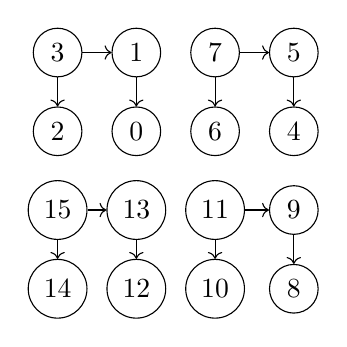
\begin{tikzpicture}[nodes={draw, circle}, ->]
        \node (3) at (0,1) {3};
        \node (1) at (1,1) {1};
        \node (0) at (1,0) {0};
        \node (2) at (0,0) {2};
        \draw [->] (3) -- (1);
        \draw [->] (3) -- (2);
        \draw [->] (1) -- (0);
        \node (7) at (2,1) {7};
        \node (5) at (3,1) {5};
        \node (4) at (3,0) {4};
        \node (6) at (2,0) {6};
        \draw [->] (7) -- (5);
        \draw [->] (7) -- (6);
        \draw [->] (5) -- (4);
        \node (11) at (2,-1) {11};
        \node (9) at (3,-1) {9};
        \node (8) at (3,-2) {8};
        \node (10) at (2,-2) {10};
        \draw [->] (11) -- (9);
        \draw [->] (11) -- (10);
        \draw [->] (9) -- (8);
        \node (15) at (0,-1) {15};
        \node (13) at (1,-1) {13};
        \node (12) at (1,-2) {12};
        \node (14) at (0,-2) {14};
        \draw [->] (15) -- (13);
        \draw [->] (15) -- (14);
        \draw [->] (13) -- (12);
\end{tikzpicture}}
\caption{\label{novel4} Illustration of novel mapping for a lattice of $4\times 4$ modes}
\end{figure}
\subsection{Theoretical improvement of this mapping} \label{theorynovel}
First, considering the Pauli weights of the vertical interactions (numbering rows from $0$):
\begin{itemlist}
\item The even rows of interactions are reduced from an average of $N + 1$ (where $N$ is the length of the lattice) to $2$\\
\item The odd rows of interactions are reduced from an average of $N + 1$ to $\frac{N-1}{4} + 6$
\end{itemlist}
Then considering the Pauli weights of the horiztonal interactions (numbering columns from $0$):
\begin{itemlist}
\item The even columns of interactions are increased from an average of $2$ to $3.5$\\
\item The odd coumns of interactions are increased from an average of $2$ to $6$
\end{itemlist}
Therefore, the overall average Pauli weight is decreased from $\frac{N}{2} + \frac{3}{2}$ to roughly $\frac{N}{8} + \frac{34}{8}$ (averaging over the even and odd rows). In reality, the average Pauli sum slightly deviates from this depending on whether there are more even rows or columns than odd. As in the case of the $20 \times 20$ lattice I computed which has more even rows than odd rows, the theory estimates a Pauli weight of approximately $6.75$ compared to the calculated value of $6.42$.
\subsection{Proposed expansion of this mapping}
We have only considered the example of $2\times 2$ cells for ease of illustration and to demonstrate the proof of principle, but generally it may be optimal to use cells of other dimensions. Further research is needed to investigate other cellular structures and determine the optimal strucutre for a given level of complexitity (as dictated by the architecture of the device). We conjecture that using a $4\times 4$ cell may prove optimal for large lattices, however, such lattices lie out of the reach of current NISQ devices due to the large qubit count required to simulate them. Even the $20 \times 20$ lattice considered above would require $400$ qubits (neglecting any requirement for error correction) which is beyond today's computers.\\\\
Additionally, this mapping was orginally concieved as a way of combining the techniques of fermionic enumeration and Bravyi-Kitaev. It may be possible to find a much more efficent overall layout for the cells than a simple S-pattern and further drastically reduce the number of gates. Further research is necessary to determine if a more optimal pattern exists, and if so how much difference it makes.
\section{Conclusion}
\raggedbottom
Accurate simulation of fermionic systems would prove very useful for a number of applications in Quantum Chemistry including determining the ground state energies of molecules. However, the large number of degrees of freedom contained in such systems make classical simulation unfeasible for large molecules. Therefore, we turn to quantum computation in order to efficently simulate fermions. One of the main challenges of simulating fermions on a quantum computer is due to their unusal non-local property of anti-symmetry under exchange. This essay has described a few different mappings from fermions to qubits that solve this problem.\\\\
As discussed in Section~\ref{vqe_section}, one of the primary measures of the effectiveness of these mappings when applied to real world problems is their locality (measured in terms of average pauli weight). Three methods for improving their locality from the naive Jordan-Wigner approach have been discussed. \\\\
The first of these (the Bravyi-Kitaev mapping) initially seemed very promising, theoretically predicted to exponentially reduce the average Pauli-weight. However, in real world simulations (discussed in Section~\ref{bravyikitavecompare}) only a constant improvement of up to 40\% in circuit length was observed (depending on the optimisation or Trotter ordering choosen). Even worse when using the optimal Trotter ordering for reducing gate count (lexicographic ordering) the Jordan-Wigner mapping outperformed the Bravyi-Kitaev for some larger molecules. Seemingly the complexity of the Bravyi-Kitaev mapping negates a large amount of its benefit and means it requires a highly connected architecture to work efficently.
\\\\
The Deby-Klassen mapping (and other `local' mappings) overwhelmingly succeed in improving the locality by lowering the average Pauli weight to a constant. However, it achieves this by sacrificing qubit count, and so is not ideal for the NISQ era with limited numbers of qubits available. Additionally, it is only useful for Hamiltonians with certain regular lattices of local interactions.\\\\
The only scheme that has been discussed which does not require any additional resources or restrictions upon the architecture is fermionic enumeration. Section~\ref{fermionic-enumeration_section} discussed how this could achieve a constant reduction in average Pauli weight of 13.9\% on a square lattice (increasing to 40\% by utilising just 2 ancilla qubits). This is approximately a similar improvement to the real world performance of the Bravyi-Kitaev mapping but without any additional requirements from the architecture. It is possible that a Jordan-Wigner transformation with optimal fermonic enumeration may perform better than the Bravyi-Kitaev mapping on real world problems, however further research is needed to test this hypothesis.\\\\\
Finally, the new mapping we have proposed allows for a trade-off between the Jordan-Wigner and the Bravyi-Kitaev mapping. We can increase the required complexity from a connected array to a connected cellular lattice (or even just a connected square lattice) and gain up to a 75\% reduction in gate count (theoretically in the limit of large lattices).  We have demonstrated that this gives a more modest but still significant reduction of 44.2\% in gate count for a $20 \times 20$ lattice, and we would expect this advantage to improve with lattice size.\\\\
In conclusion, if we were tasked with picking an optimium fermion-to-qubit mapping to perform quantum phase estimation on a square lattice, we would pick the Jordan-Wigner mapping with Mitchison-Durbin enumeration. We would prefer this over the more gate efficent Derby-Klassen (or other `local' mappings) as in the NISQ era, with limited numbers of qubits available, we must prioritise qubit count. The decision to rank it above Bravyi-Kitaev is primarily due to reducing the architecture requirements, as NISQ devices often have limited connectivity. These concerns about architecture outstrip the theoretical potential for gate reduction as Section~\ref{bravyikitavecompare} discussed. Lastly, we would select it over the novel mapping which is untested and enforces additional restrictions on the connectivity. However, with more research into this new mapping, such as applying enumeration schemes and optimising the cell size, it could potentially outperform the Jordan-Wigner mapping with Mitchison-Durbin enumeration.  
\pagebreak
        \section{References}
\begin{thebibliography}{000}
        \bibitem{feynmann} Feynman, R.P.. {\it Simulating physics with computers}. International Journal of Theoretical Physics 1982;21(6-7):467–488. \url{doi:10.1007/bf02650179}.
        \bibitem{originalJordanWigner} Pascual Jordan and Eugene Wigner. {\it  {\"U}ber das Paulische {\"A}quivalenzverbot}. Zeitschrift fur Physik, 47(9-10):631{651, September 1928.
                \bibitem{fermionicEncoding} Chiew, M. and Strelchuk, S.. {\it Optimal Fermion-Qubit Mappings}. ArXiv:2110.12792 [Quant-Ph], 25 October 2021. \url{http://arxiv.org/abs/2110.12792}
                \bibitem{vqe}
                Tilly, Jules, Hongxiang Chen, Shuxiang Cao, Dario Picozzi, Kanav Setia, Ying Li, Edward Grant, et al. {\it The Variational Quantum Eigensolver: A Review of Methods and Best Practices}. ArXiv:2111.05176 [Quant-Ph], 9 November 2021. \url{http://arxiv.org/abs/2111.05176} \textbf{look for journal version}
                \bibitem{chemistryReview} McArdle, Sam, Suguru Endo, Alán Aspuru-Guzik, Simon C. Benjamin, and Xiao Yuan. {\it Quantum Computational Chemistry}. Reviews of Modern Physics 92, no. 1 (30 March 2020): 015003. \url{https://doi.org/10.1103/RevModPhys.92.015003}.
                \bibitem{nielsenChuang} Nielsen, M.A., Chuang, I.L.. {\it Quantum Computation and Quantum Information}. Cambridge: Cambridge University Press; 2009. ISBN
                \bibitem{seeley} Seeley, Jacob T., Martin J. Richard, and Peter J. Love. {\it The Bravyi-Kitaev Transformation for Quantum Computation of Electronic Structure}. The Journal of Chemical Physics 137, no. 22 (14 December 2012): 224109. \url{https://doi.org/10.1063/1.4768229}.

9780511976667. doi:10.1017/cbo9780511976667. 
\bibitem{suzuki} Suzuki, Masuo. {\it Generalized Trotter’s Formula and Systematic Approximants of Exponential Operators and Inner Derivations with Applications to Many-Body Problems}. Communications in Mathematical Physics 51, no. 2 (June 1976): 183–90. \url{https://doi.org/10.1007/BF01609348}.
\bibitem{bravyikitaev} Bravyi, Sergey, and Alexei Kitaev. {\it Fermionic Quantum Computation}. Annals of Physics 298, no. 1 (May 2002): 210–26. \url{https://doi.org/10.1006/aphy.2002.6254}.
\bibitem{tranter2018} Tranter, Andrew, Peter J. Love, Florian Mintert, and Peter V. Coveney. {\it A Comparison of the Bravyi-Kitaev and Jordan-Wigner Transformations for the Quantum Simulation of Quantum Chemistry}. Journal of Chemical Theory and Computation 14, no. 11 (13 November 2018): 5617–30. \url{https://doi.org/10.1021/acs.jctc.8b00450}.
\bibitem{operatorLocality} Havlíček, Vojtěch, Matthias Troyer, and James D. Whitfield. {\it Operator Locality in Quantum Simulation of Fermionic Models}. Physical Review A 95, no. 3 (29 March 2017): 032332. \url{https://doi.org/10.1103/PhysRevA.95.032332}.
\bibitem{superfast} Setia, Kanav, Sergey Bravyi, Antonio Mezzacapo, and James D. Whitfield. {\it Superfast Encodings for Fermionic Quantum Simulation}. Physical Review Research 1, no. 3 (18 October 2019): 033033. \url{https://doi.org/10.1103/PhysRevResearch.1.033033}.
\bibitem{derbyklassen} Derby, Charles, and Joel Klassen. {\it A Compact Fermion to Qubit Mapping}. Physical Review B 104, no. 3 (8 July 2021): 035118. \url{https://doi.org/10.1103/PhysRevB.104.035118}.
\bibitem{derbyklassen2} Derby, Charles, and Joel Klassen. {\it A Compact Fermion to Qubit Mapping Part 2: Alternative Lattice Geometries}. ArXiv:2101.10735 [Quant-Ph], 26 January 2021. http://arxiv.org/abs/2101.10735.
\bibitem{edgesum} Garey, M. R., D. S. Johnson, and L. Stockmeyer. {\it Some Simplified NP-Complete Graph Problems}. Theoretical Computer Science 1, no. 3 (1 February 1976): 237–67. \url{https://doi.org/10.1016/0304-3975(76)90059-1}.
\bibitem{mitchisondurbin} Mitchison, Graeme, and Richard Durbin. {\it Optimal Numberings of an $N \times N$ Array}. SIAM Journal on Algebraic Discrete Methods 7, no. 4 (1 October 1986): 571–82. \url{https://doi.org/10.1137/0607063}.
\bibitem{reducequbits} Moll, Nikolaj, Andreas Fuhrer, Peter Staar, and Ivano Tavernelli. {\it Optimizing Qubit Resources for Quantum Chemistry Simulations in Second Quantization on a Quantum Computer}. Journal of Physics A: Mathematical and Theoretical 49, no. 29 (22 July 2016): 295301. \url{https://doi.org/10.1088/1751-8113/49/29/295301}.
\bibitem{me}
                \bibitem{first}
P. Horodecki and R. Horodecki (2001), {\it Distillation and bound entanglement},
Quantum Inf. Comput., Vol.1, pp. 045-075.

\bibitem{cal}
R. Calderbank and P. Shor (1996), {\it Good quantum error
       correcting codes exist},
Phys. Rev. A, 54, pp. 1098-1106.

\bibitem{niel}
M.A. Nielsen and J. Kempe (2001), {\it Separable states are
more disordered globally than locally}, quant-ph/0105090.

\bibitem{mar}
A.W. Marshall and I. Olkin (1979), {\it Inequalities: theory of majorization and its applications},
Academic Press (New York).

\bibitem{chenxu} Chen, Yu-An, and Yijia Xu. ‘Equivalence between Fermion-to-Qubit Mappings in Two Spatial Dimensions’. ArXiv:2201.05153 [Cond-Mat, Physics:Math-Ph, Physics:Quant-Ph], 13 January 2022. \url{http://arxiv.org/abs/2201.05153}

\bibitem{chen2} Chen, Yu-An, Anton Kapustin, and Djordje Radicevic. ‘Exact Bosonization in Two Spatial Dimensions and a New Class of Lattice Gauge Theories’. Annals of Physics 393 (June 2018): 234–53. \url{https://doi.org/10.1016/j.aop.2018.03.024}

\bibitem{codes} Steudtner, Mark, and Stephanie Wehner. ‘Quantum Codes for Quantum Simulation of Fermions on a Square Lattice of Qubits’. Physical Review A 99, no. 2 (8 February 2019): 022308. \url{https://doi.org/10.1103/PhysRevA.99.022308}
\bibitem{chiew2} Chiew, Mitchell, and Sergii Strelchuk. ‘Optimal Fermion-Qubit Mappings’. ArXiv:2110.12792 [Quant-Ph], 2 February 2022. \url{http://arxiv.org/abs/2110.12792}
\bibitem{fenwick} Fenwick, Peter M. ‘A New Data Structure for Cumulative Frequency Tables’. Software: Practice and Experience 24, no. 3 (March 1994): 327–36. \url{https://doi.org/10.1002/spe.4380240306}
\bibitem{noiseerror} Sawaya, Nicolas P. D., Mikhail Smelyanskiy, Jarrod R. McClean, and Alán Aspuru-Guzik. ‘Error Sensitivity to Environmental Noise in Quantum Circuits for Chemical State Preparation’. Journal of Chemical Theory and Computation 12, no. 7 (12 July 2016): 3097–3108. https://doi.org/10.1021/acs.jctc.6b00220.
\bibitem{tilly} Tilly, Jules, Hongxiang Chen, Shuxiang Cao, Dario Picozzi, Kanav Setia, Ying Li, Edward Grant, et al. ‘The Variational Quantum Eigensolver: A Review of Methods and Best Practices’. ArXiv:2111.05176 [Quant-Ph], 9 November 2021. \url{http://arxiv.org/abs/2111.05176}.
\bibitem{firstech1} Abrams, Daniel S., and Seth Lloyd. ‘Simulation of Many-Body Fermi Systems on a Universal Quantum Computer’. Physical Review Letters 79, no. 13 (29 September 1997): 2586–89. \url{https://doi.org/10.1103/PhysRevLett.79.2586}.
\bibitem{firstech2} Berry, Dominic W., Mária Kieferová, Artur Scherer, Yuval R. Sanders, Guang Hao Low, Nathan Wiebe, Craig Gidney, and Ryan Babbush. ‘Improved Techniques for Preparing Eigenstates of Fermionic Hamiltonians’. Npj Quantum Information 4, no. 1 (December 2018): 22. \url{https://doi.org/10.1038/s41534-018-0071-5}
\bibitem{barrenplat} Cerezo, M., Akira Sone, Tyler Volkoff, Lukasz Cincio, and Patrick J. Coles. ‘Cost Function Dependent Barren Plateaus in Shallow Parametrized Quantum Circuits’. Nature Communications 12, no. 1 (December 2021): 1791. \url{https://doi.org/10.1038/s41467-021-21728-w}.
\end{thebibliography}

\end{document}

